%%
%%AASTeX requires revtex4-1.cls (http://publish.aps.org/revtex4/) and
%% other external packages (latexsym, graphicx, amssymb, longtable, and epsf).

%% using aastex version 6.2
\documentclass[twocolumn]{aastex62}
\usepackage{color,comment}
\usepackage[normalem]{ulem}
\usepackage[caption=false]{subfig}

\newcommand{\red}[1]{{\textcolor{red}{#1}}}
\newcommand{\green}[1]{{\textcolor{green}{#1}}}
\newcommand{\vdag}{(v)^\dagger}
\newcommand\aastex{AAS\TeX}
\newcommand\latex{La\TeX}
%\usepackage{float}
\usepackage{wrapfig}

\graphicspath{{./}}

%% Reintroduced the \received and \accepted commands from AASTeX v5.2
\received{}
\revised{}
\accepted{\today}
%% Command to document which AAS Journal the manutextttript was submitted to.
%% Adds "Submitted to " the arguement.
%\submitjournal{ApJ}


%%%%%%%%%%%%%%%%%%%%%%%%%%%%%%%%%%%%%%%%%%%%%%%%%%%%%%%%%%%%%%%%%%%%%%%%%%%%%%%%
%%
%% The following section outlines numerous optional output that
%% can be displayed in the front matter or as running meta-data.
%%
%% If you wish, you may supply running head information, although
%% this information may be modified by the editorial offices.
\shorttitle{Estimating Stellar Masses}
\shortauthors{S. Lower et al.}
%%
%% You can add a light gray and diagonal water-mark to the first page 
%% with this command:
% \watermark{text}
%% where "text", e.g. DRAFT, is the text to appear.  If the text is 
%% long you can control the water-mark size with:
%  \setwatermarkfontsize{dimension}
%% where dimension is any recognized LaTeX dimension, e.g. pt, in, etc.
%%
%%%%%%%%%%%%%%%%%%%%%%%%%%%%%%%%%%%%%%%%%%%%%%%%%%%%%%%%%%%%%%%%%%%%%%%%%%%%%%%%


\begin{document}

\title{How Well Can We Measure the Stellar Mass of a Galaxy? \\ Ground-Truthing SED Fitting Methods with Cosmological Simulations
}



%co authors: desika, joel, ben, charlie, romeel, others?
\author{Sidney Lower}
\affil{Department of Astronomy, University of Florida}

\author{Desika Narayanan}
\affil{Department of Astronomy, University of Florida}
\affil{University of Florida Informatics Institute}
\affil{Cosmic Dawn Center at the Niels Bohr Institute, University of Copenhagen and DTU-Space, Technical University of Denmark}
\author{Joel Leja}
\affil{Center for Astrophysics | Harvard \& Smithsonian}
\author{Benjamin Johnson}
\affil{Center for Astrophysics | Harvard \& Smithsonian}
\author{Charlie Conroy}
\affil{Center for Astrophysics | Harvard \& Smithsonian}
\author{Romeel Dav{\'{e}}}
\affil{Institute for Astronomy, Royal Observatory, Univ. of Edinburgh}


\begin{abstract}

The stellar mass ($M_*$) of a galaxy is one of the most robust quantities estimated with spectral energy distribution (SED) modeling, but the technique rests on assumptions concerning a galaxy's star formation history and dust attenuation law that are detrimental to this robustness.  Classically, star formation histories (SFHs) are modeled with simplified parameterized functional forms, but these forms are unlikely to capture the true diversity of galaxy SFHs and may impose systematic uncertainties and biases on results. Recently, non-parametric SFH models have shown promise in marginalizing over some of these uncertainties. Here, we examine the efficacy of these SFHs by ground-truthing them against mock observations of high-resolution cosmological hydrodynamic galaxy formation simulations. We demonstrate that ,when using non parameteric star formation histories, stellar masses can be estimated with greatly improved accuracy over traditional parametric SFH models, with uncertainties falling below the previously inescapable ‘factor of 2’ that has historically plagued stellar mass estimates. We also demonstrate the impact on our understanding of the evolution of the unexplained mismatch between the theoretical and observed SFR-$M_*$ relation in galaxies, with improved estimates of both stellar ages and star formation rates. 

\end{abstract}


\section{Introduction} \label{sec:intro}

The ability to accurately estimate the physical quantities of galaxies is critical for our understanding of galaxy formation and evolution. Modeling the ultraviolet (UV) to infrared (IR) spectral energy distributions (SEDs) of is one of the main diagnostics used to understand the physical characteristics of galaxies, as we can go from the observed integrated light of a galaxy to properties like stellar mass (M$_*$), star formation rate (SFR), and stellar age. The basic components in an SED model include information about stellar populations (the stellar initial mass function (IMF), stellar isochrones and spectral templates, and star formation history (SFH)) and dust (emission and attenuation). The robustness of an SED model and our ability to accurately
recover physical properties of a galaxy depend on our confidence in each model component to accurately capture the complexity of the many physical processes that occur in a galaxy and the equally complex growth history of a galaxy. There are many models that exist for each component, both empirical and theoretical. Yet the efficacy of SED modelling techniques is not well tested, at least systematically (see reviews by \cite{conroy_modeling_2013}; \cite{walcher_fitting_2011}). Measuring galaxy physical properties, especially for galaxies at high-redshift, is highly sensitive to the SED modeling technique and the level of accuracy by which one can derive these properties is still unknown \citep{hayward_should_2015}. Comparisons between SED models and fitting codes tend to highlight the systematic uncertainties that plague models for stellar evolution, star formation history, and dust attenuation (\cite{hunt_comprehensive_2019}; \cite{mitchell_how_2013}; \cite{pforr_recovering_2012}), but without a way to ground-truth these results, we cannot know for sure how accurate these models are. Recently, \cite{katsianis_high_2020} conducted a study comparing the SFR and stellar mass estimates derived from various methods including SED modeling. Using the \texttt{EAGLE} simulation (\cite{schaye_eagle_2015}; \cite{crain_eagle_2015}; \cite{mcalpine_eagle_2016}) with \texttt{SKIRT} radiative transfer (\cite{baes_radiative_2003}; \cite{baes_efficient_2011}; \cite{camps_skirt_2015}), the authors found that SFRs and stellar masses derived from SED modeling tend to be underestimated for galaxies up to redshift z=4. This has a profound impact on the implied SFR-(M$_*$) relation, or the star forming main sequence (SFMS), creating a source of tension between the derived SFMS from observations and from simulations; the tension could be due primarily to biases in the techniques used to measure these quantities instead of incorrect physics included in the simulations. Understanding the source of these mismatches can alleviate these tensions. 


The core of SED modeling lies in our ability to transform the observed light from a galaxy into physical properties like stellar mass. To estimate stellar mass, numerous assumptions must be made prior to fitting an SED model to observed data. These assumptions - the IMF, SFH, dust attenuation curve, etc. - all affect the estimated stellar mass in multiple ways and the uncertainties associated with them. The degeneracies at work between parameters like stellar age and reddening from dust attenuation, combined with over simplified models for (e.g.) the star formation history and dust attenuation curve complicate the interpretation from current SED modeling techniques. 

Let us take, for example, the star formation history model in SED fitting codes. The most common models for SFHs are parametric in form, meaning they are described by some simplified functional form and the parameters varied in the SED fit describe that functional form. Examples include the $\tau$ and delayed-$\tau$ models, which model the SFH as exponentially declining with some characteristic $e$-folding time. Although these models are computationally efficient, the restricted nature of the functional forms is unlikely to match the diversity of true galaxy SFHs. Additionally, the physical properties estimated from these parametric SFHs can be severely biased by the imposed functional form and the indirect influence of the SFH parameter priors, resulting in biased estimations and underestimated uncertainties of physical properties (\cite{simha_parametrising_2014}; \cite{iyer_reconstruction_2017}; \cite{salmon_relation_2015}; \cite{carnall_how_2019}). For instance, \cite{bisigello_statistical_2019} found that stellar mass estimates from the \texttt{LePhare} SED fitting code fit to mock observations with JWST NIRcam photometry deviate from true stellar mass estimates up to 0.8 dex, due to various model degeneracies. Similarly, \cite{curtis-lake_modelling_2020} found that the SFR-(M$_*$) relation is sensitive to the priors used in a delayed-$\tau$ SFH employed in SED modeling. The priors act to falsely narrow constraints in the SFR-stellar mass relation, resulting in underestimated uncertainties, as the constraints placed on stellar mass and SFR are better than in reality. Nonetheless, SED modeling done in the literature typically assumes a simple parametric form for the SFH.  

Parametric SFHs with more complexity have also been explored in the literature (e.g. \cite{pacifici_relative_2012}; \cite{simha_parametrising_2014}; \cite{ciesla_sfr-_2017}). An example is a log-normal parametrization, which was seen to be a good fit to Illustris galaxy SFHs \citep{diemer_log-normal_2017}. However, as shown in \cite{carnall_how_2019} and \cite{leja_how_2019}, the log-normal parametrization still suffers from the mismatches in stellar age as the more simple parametric forms, as the duration of star formation is a model variable so the derived ages are younger on average than the truth. The added complexity of these models is still hindered by the choice of prior distributions on model parameters, such that the added flexibility does not afford greater freedom from biases and uncertainties. 


A clear example of the impact of these prior assumptions is presented in \citet{michalowski_stellar_2012}, in which the authors estimated the stellar masses of high-$z$ dust star forming galaxies. These authors found that the assumed star formation history model had the largest affect on the uncertainty in the estimated stellar masses for observations of sub-millimeter galaxies (SMGs) from the literature. Similarly \cite{dudzeviciute_alma_2019} found that the difference between the estimated stellar masses predicted by the \texttt{MAGPHYS} SED fitting software and true stellar masses for galaxies from the \texttt{EAGLE} cosmological galaxy formation simulation was close to $0.5$ dex, consistent with the uncertainties in \citet{michalowski_stellar_2012} SMG stellar mass estimates and attributed this offset to the SFH model used.

Recently, a series of models employing non-parametric forms for galaxy star formation histories in SED modeling have been developed to minimize the uncertainties propagated by the use of more simplified parametric models such as the $\tau$ model.  These non-parametric SFH models have been shown to have the flexibility to reasonably reproduce the variation in SFHs seen in observations and cosmological simulations. These SFH models are non-parametric in the sense that they are not restricted to a particular functional form. Some non-parametric SFHs are modeled as a function of families of SFHs that effectively cover the space of all physical SFHs, as developed in \cite{iyer_reconstruction_2017} and improved upon in \cite{iyer_nonparametric_2019} with the Dense Basis method. Other methods go a step further and model the SFH of a galaxy as multiple bins of constant star formation rate, effectively removing any constraints from a functional form, as developed in \cite{leja_deriving_2017} and expanded and improved upon in \cite{leja_how_2019} and \cite{leja_older_2019}. These models are described by priors on both the shape and normalization of the SFH. The shape of the SFH is informed by a certain prior and the overall normalization of the SFH informed by another, so that each component is effectively independent of the other.   

While the aforementioned authors explored the impact of non-parametric star formation histories on their observational data sets, the method is yet to be ground truthed against the true stellar mass of the galaxy. An important avenue to explore is therefore the ability of these non-parametric SFHs to recover both the stellar mass of a galaxy and the true SFH. To that end, we employ mock 'observations' of galaxies from cosmological hydrodynamic galaxy formation simulations to both test and tune the parameters used to estimate these quantities. We also compare the abilities of the non-parametric SFH models to the traditional parametric forms used and show that the non-parametric models are able to recover the observed star forming main sequence with much improved accuracy.   


\section{\texttt{simba} Cosmological Simulation} 
\label{section:simulations}

\begin{figure*}
    \centering
    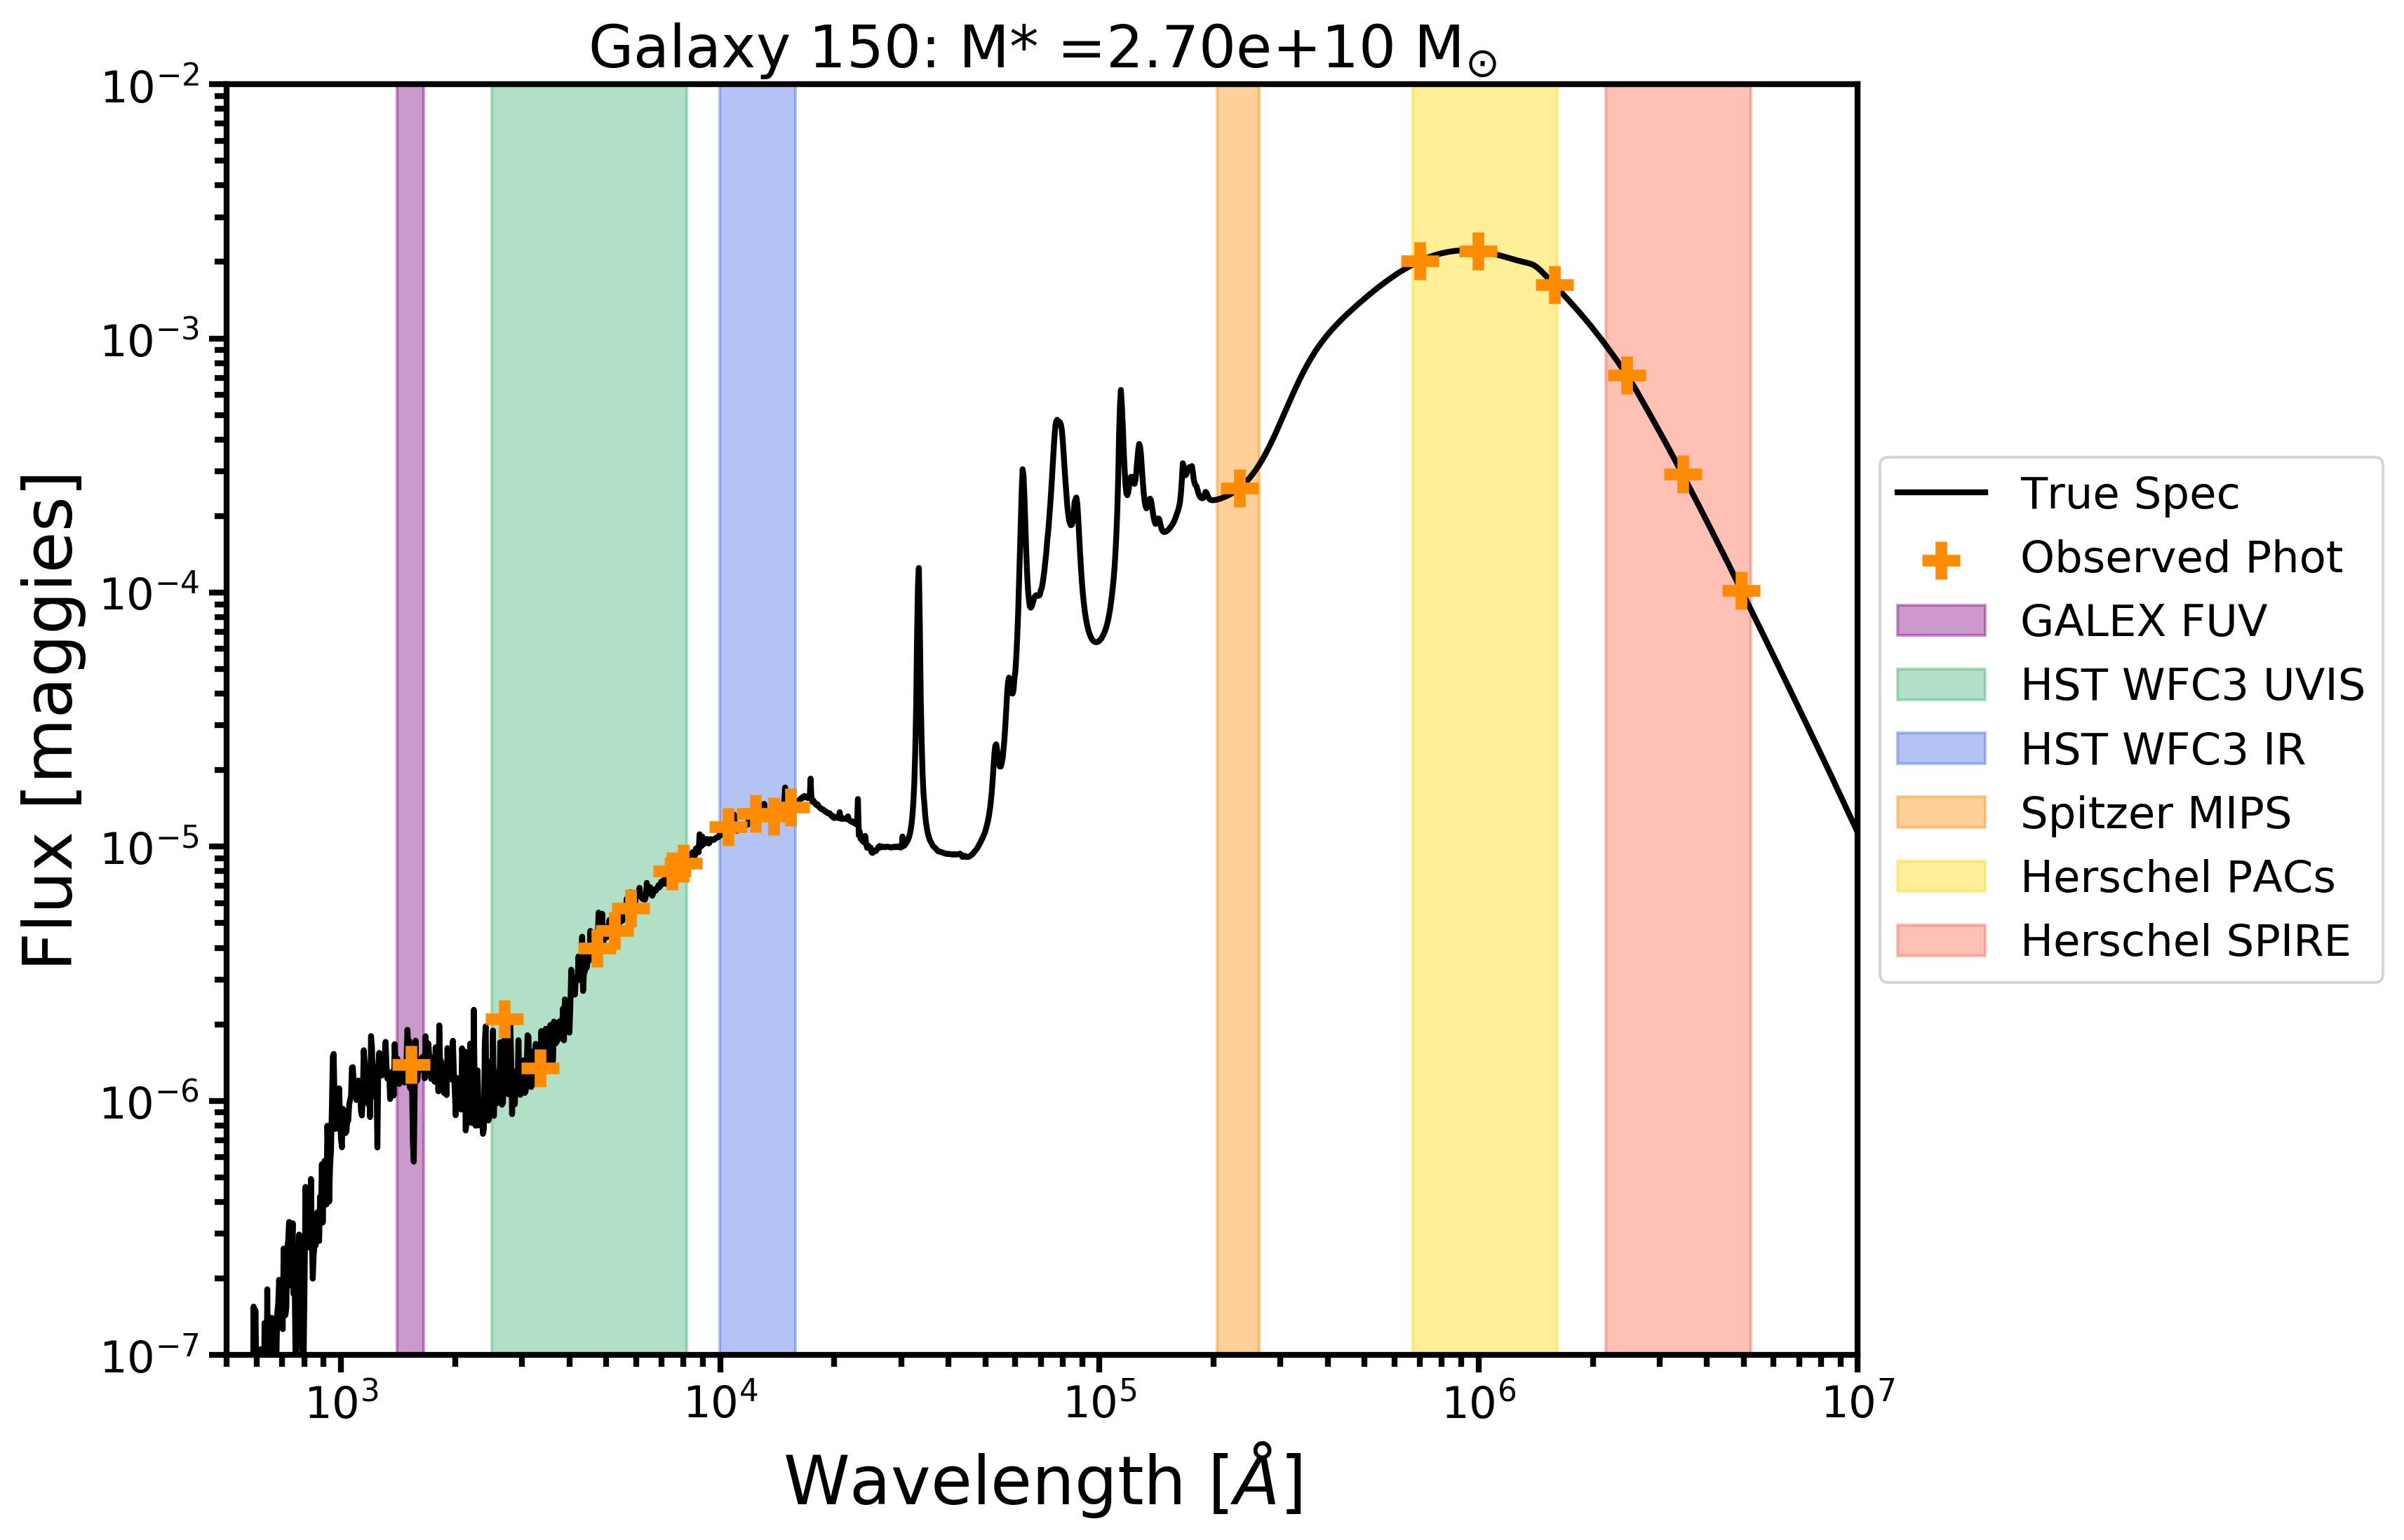
\includegraphics[width = \textwidth]{fancySED_150.png}
    \caption{Example \texttt{powderday} mock SED with 'observed' photometric bands highlighted, spanning from \textit{GALEX FUV} to \textit{Herschel SPIRE}, totaling 19 bands resulting in almost complete coverage across all wavelength regimes. All galaxies are observed with the same filters, and photometric errors are fixed at $3\%$. Photometry is 'observed' for each filter and convolved over the filter bandwidth. NIR photometry spanning from $\sim$2$\mu$m to 20$\mu$m is ignored due to the unreliability of \texttt{powderday} PAH templates.}
    \label{fig:SED}
\end{figure*}

To assess the validity of various star formation history models, we utilize cosmological simulations to ground-truth the predictions made by each model (stellar mass, mass-weighted age, and star formation rate). We use the \texttt{simba} cosmological simulation, described in full in \cite{dave_simba:_2019}. Briefly, \texttt{simba} is the descendant of the simulation suite \texttt{mufasa} and relies on \texttt{gizmo}'s meshless finite mass hydrodynamics. New subresolution prescriptions for stellar and AGN feedback as well as black hole growth have enabled \texttt{simba} to more accurately reproduce observables like the galaxy stellar mass function and the star forming main sequence. We use a 25 Mpc h$^{-1}$ size with 512$^3$ particles, resulting a mass resolution of 1.4$\times$ 10$^6 \: \mathrm{M}_{\odot}$. We use \texttt{caesar}\footnote{https://github.com/dnarayanan/caesar} to identify galaxies using a 6D friends-of-friends algorithm. Around 2500 galaxies are found in the redshift z=0 snapshot. The largest galaxy at z=0 has stellar mass of 1.4$\times$ 10$^{12} \: \mathrm{M}_{\odot}$. 

Post-processing radiative transfer is performed by \texttt{powderday}\footnote{https://github.com/dnarayanan/powderday}. \texttt{Powderday} wraps \texttt{FSPS} stellar population synthesis (\cite{conroy_propagation_2009}; \cite{conroy_propagation_2010}) and the \texttt{python} bindings \texttt{python-fsps} and \texttt{hyperion} dust radiative transfer (\cite{robitaille_hyperion:_2011}, resulting in model synthetic SEDs spanning from the UV to submilimeter wavelengths. The additional implementation of a model for the production, growth, and destruction of dust grains in \texttt{simba} (\cite{li_dust--gas_2019}) allows for a more realistic treatment of dust attenuation and emission from galaxies. 

We generate mock photometry from the synthetic \texttt{powderday} SEDs. Photmetry spans from \textit{GALEX FUV} filter at 1542 {\AA} to the \textit{Herschel SPIRE} band at 500 $\mu$m as shown in \ref{fig:SED}. We fixed uncertainties to 3\% of the flux value, since the aim of this study is not to analyze the affect of photometric uncertainties but rather the systematics that arise from the use of various SFH models. Though the assumptions made when modeling stellar spectra and isochrones, especially concerning the impact of late stellar evolutionary stages on a galaxy's SED, are important and the physical parameters derived from SED can be greatly influenced by these assumptions, they are ultimately outside the scope of this paper. 



\section{SED Fitting}


In order to model the mock SEDs generated by \texttt{powderday} from our galaxy formation simulations, we use the Bayesian inference code \texttt{prospector}\footnote{https://github.com/bd-j/prospector} (\cite{leja_deriving_2017}; \cite{leja_how_2019}). \texttt{Prospector} derives galaxy physical properties by using stellar population synthesis evolved with dust within the framework of \texttt{FSPS}. As both \texttt{powderday} and \texttt{prospector} use \texttt{FSPS} with the same spectral libraries (MILES) and isochrones (MIST) for stellar population synthesis, uncertainties involved with stellar evolution are minimal. (Models for AGN and nebular emission are also included in \texttt{Prospector} but were not used with this study as the these components were ignored in the post-processes radiative transfer). \texttt{Prospector} uses a Bayesian framework via \texttt{dynesty} nested sampling (\cite{speagle_dynesty:_2019}) to fit the observed SEDs and provide posterior distribution estimates of physical parameters such as stellar mass, stellar metallicity, and star formation rate. The power of \texttt{dynesty} lies in its ability to efficiently sample multi-model distributions and have well-defined stopping criteria based evaluations of Bayesian evidence ensuring model convergence.


\subsection{Star Formation History}

One of the main components in SED modeling is how to handle stellar evolution. This includes assumptions about the stellar initial mass functions, stellar metallicities, evolutionary tracks, and the aggregate star formation history of a galaxy. The effect of the assumed IMF in SED modeling is much debated, but is outside the scope of this analysis; instead, we note that both \texttt{powderday} and \texttt{prospector} assume the same IMF. The focus of this analysis is instead on the impact of the assumed form of the star formation history. Recently, models for non-parametric SFH models have been developed in order to offer a greater flexibility in matching true galaxy SFHs as they are not biased towards a certain shape (i.e. increasing/decreasing star formation over time). Instead these SFHs move significantly beyond the simplified parametric models that have been used by the community for decades in that they simultaneously evolve multiple bins of a constant star formation rate, effectively removing any constraints from a functional form. The non-parametric models are constrained by priors that can either enforce continuity (i.e. the SFH is smooth rather than bursty) or that allow for episodes of SF bursts. An example of these models (and the other parametric models used in this paper) is shown in Figure \ref{fig:sfh_ex}. The non-parametric star formation histories used in this analysis are described in depth in \citet{leja_how_2019}, while we provide a more top level view in the following sections. 



\subsubsection{Parametric Forms}

As a means for comparison, three simple parametric star formation histories were considered:

\textbf{Delayed$-\tau$ model}: The delayed-$\tau$ model is an exponentially declining SFH, parameterized by the $e$-folding time that is informed by a log-uniform prior. The free parameters for this model also include the stellar mass formed by the galaxy and the maximum age of the stellar population. 

\textbf{Delayed$-\tau$ model + burst}: This is a the same as above but including a random burst of star formation. During a burst, some fraction of mass is formed in an instantaneous burst of star formation. 

\textbf{Constant}: A constant star formation history is primarily used in the literature as a proxy for recent star-burst activity or to model star forming galaxies at high redshift. 


\subsubsection{Non-parametric Forms}
\label{section:dirichlet}

The two non-parametric SFH models as developed in \cite{leja_deriving_2017} are constrained by different priors but are similarly implemented in \texttt{prospector}. In practice, the fractional mass formed in each time bin is fit for independently of the total mass formed (i.e. the shape of the SFH is separate from the normalization). 

\textbf{Dirichlet prior}: For this model, the marginal probability distribution on each specific star formation rate follows a Dirichlet prior, which is multivariate beta distribution. The time bins can be adjusted in both number and size by the user, but remain fixed during the fit. Where photometric data fails to constrain the star forming history of the galaxy, a constant star formation history is recovered. An additional parameter, called the concentration parameter, is required to fit the SFHs and controls the concentration of stellar mass formation across time bins. Lower concentration values result in more bursty star formation histories, while higher values result in smoother SFHs. A value of $0.7$ was used for these fits, allowing for moderate bursts of star formation. 

\textbf{Continuity prior}: The continuity star formation history models the SFH as constant in certain time intervals (number and size adjustable by the user) with normalization informed by a continuity prior, such that sharp changes in the star formation rate across time intervals are weighted against. The continuity prior, described by the Student's$-$t distribution, informs the difference in adjacent star formation rates ($\mathrm{log}(SFR_n / SFR_{n+1})$). 

Though distinction between the two non-parametric models is made here for clarity, the following analysis will focus on just one model constrained by the Dirichlet prior. This choice was made to accommodate the stochastic behavior of the \texttt{simba} galaxies (known a priori to this analysis) and to reserve comparisons between the two constraints, which are outside the scope of this paper. Thus, throughout this paper, we will refer to this SFH model simply as 'non-parametric.' 


\begin{figure}[h]

\centering
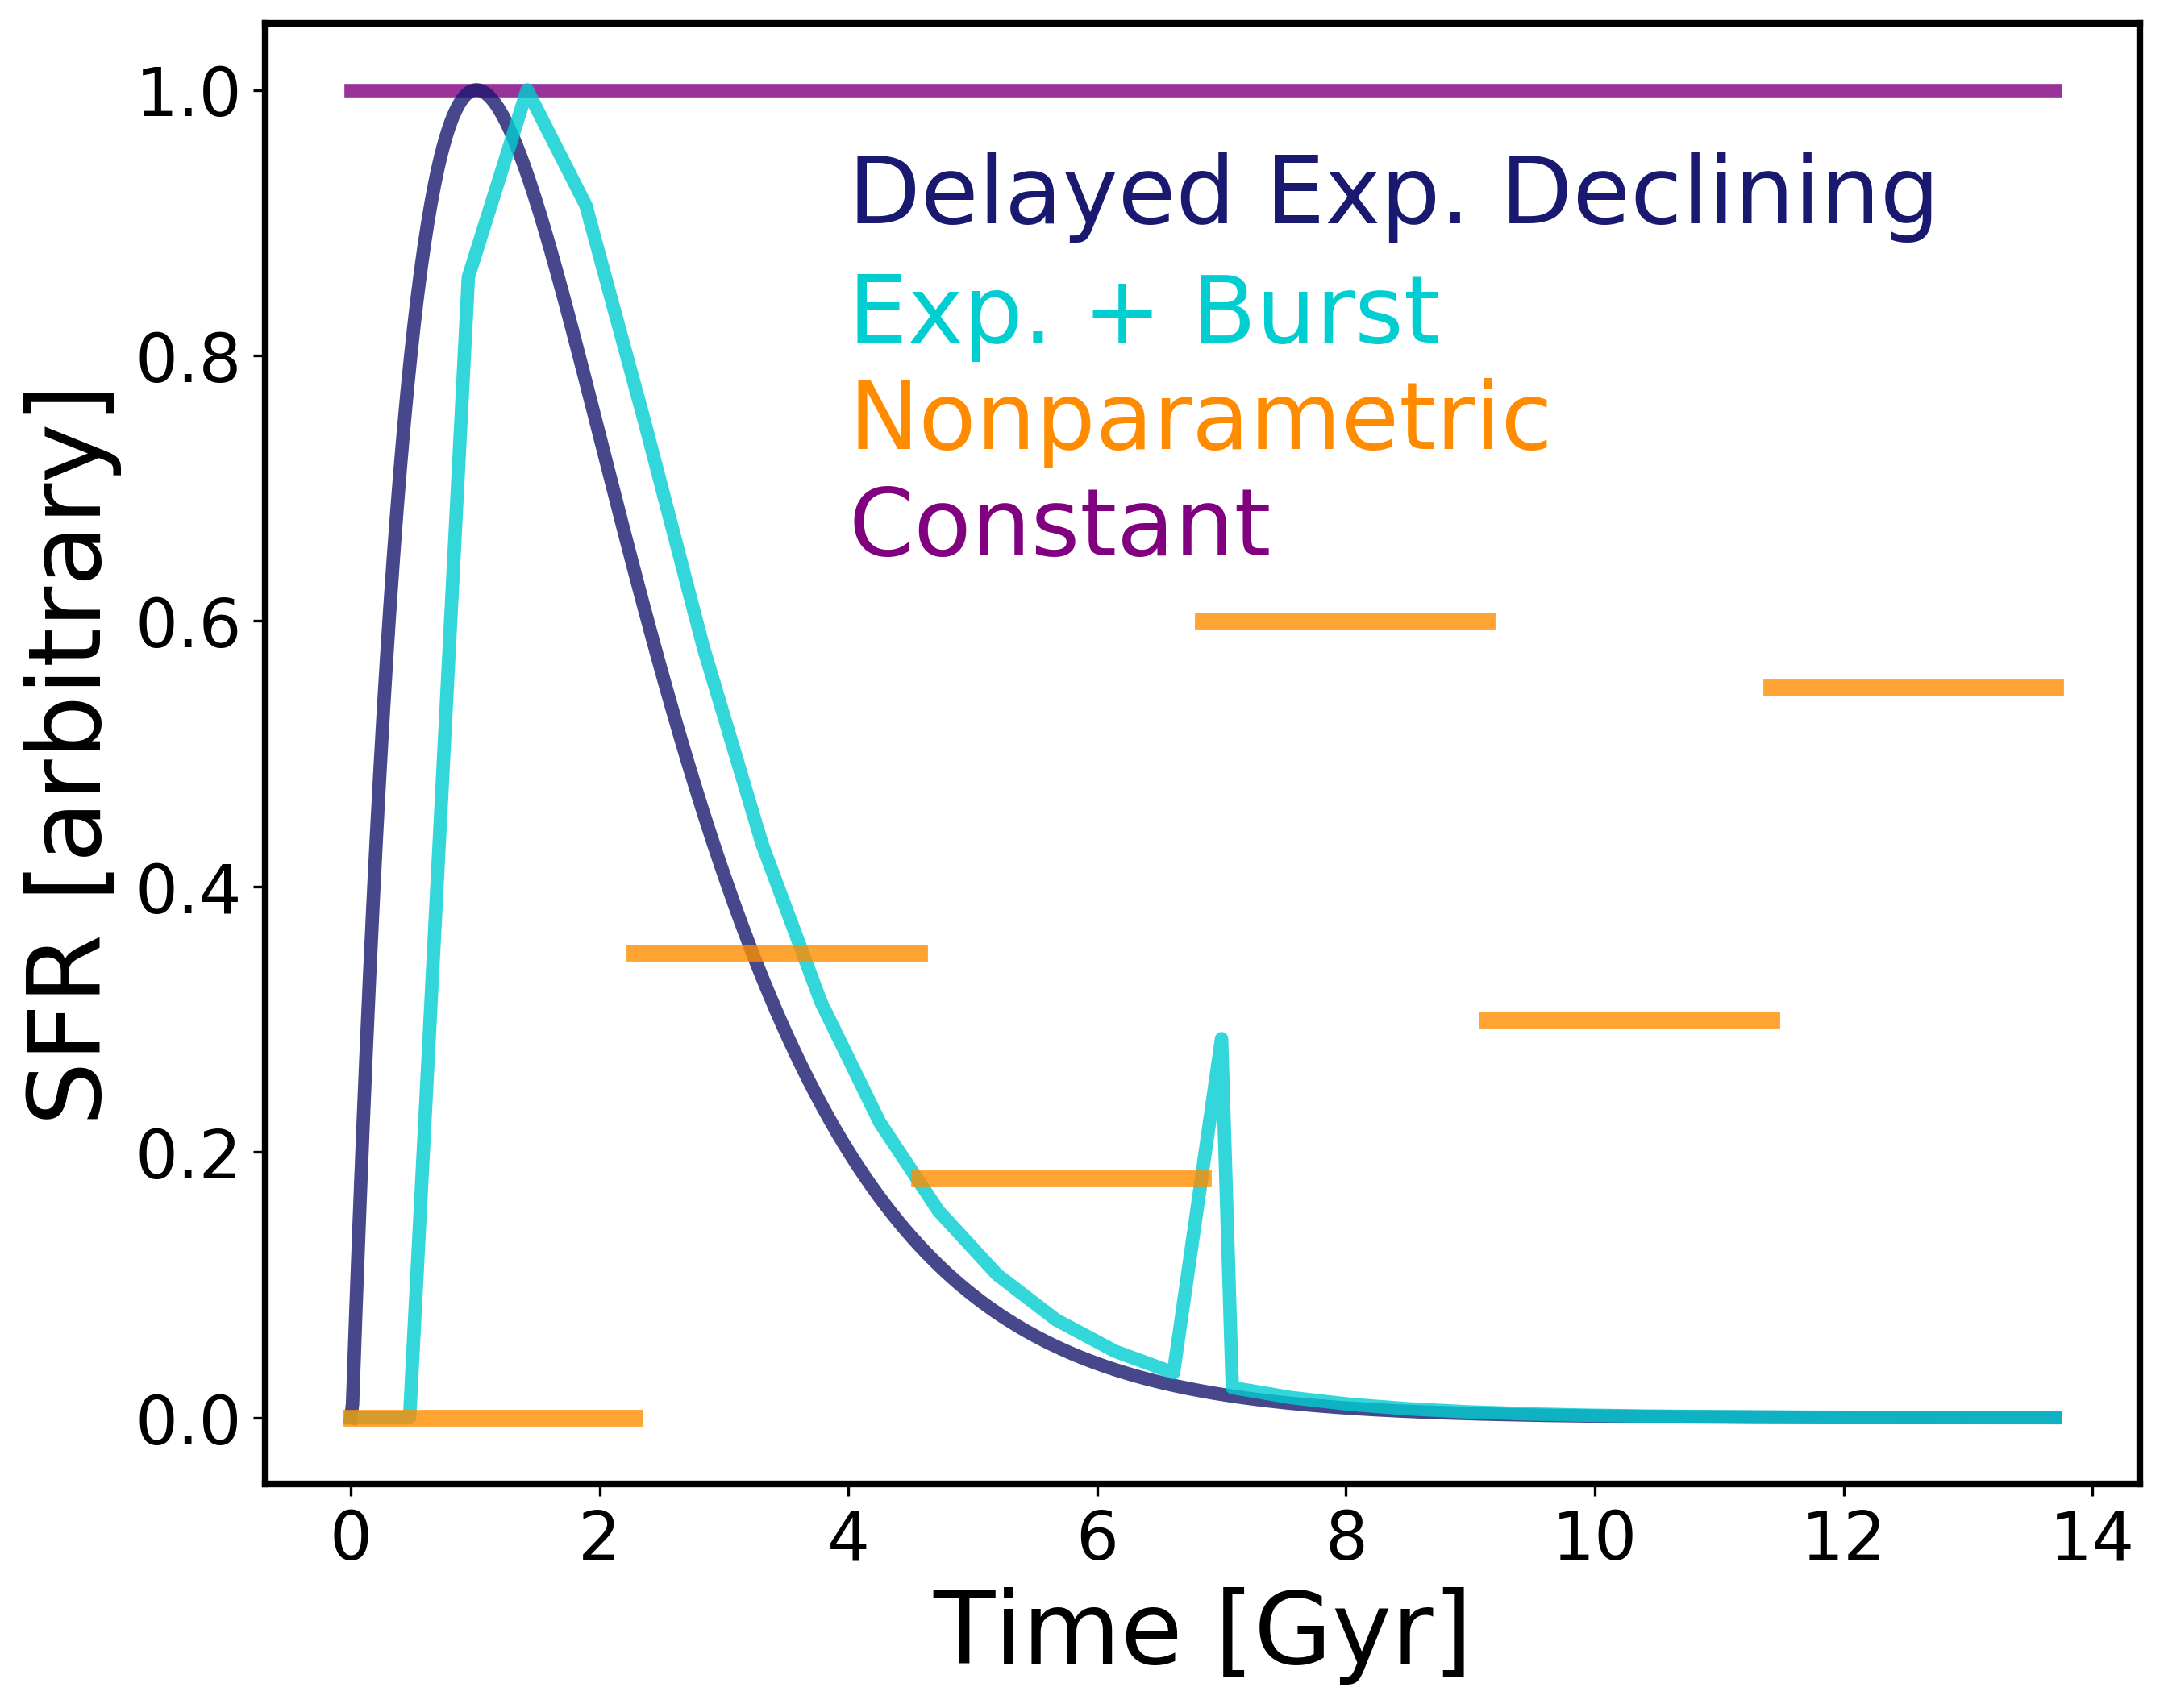
\includegraphics[width=0.5\textwidth]{sfh.png}\hfill

\caption{Example star formation history models considered in this paper (curves are of arbitrary galaxy parameters and are normalized). The parametric models include the declining exponential models which peak at some time and decline exponentially afterwards (delayed$-\tau$ and delayed$-\tau$ plus a burst component), and a constant star formation rate across time. The non-parametric models are implemented as bins of constant star formation that can vary in number and are simultaneously varied in the SED fit, constrained by a choice of two priors that can enforce a degree of continuity in the SFH. }
\label{fig:sfh_ex}

\end{figure}
 



\subsection{Metallicity and Dust}

We use the same metallicity and dust models regardless of star formation history model. This allows us to isolate uncertainties related to the SFH so any differences in stellar mass result from just the chosen SFH model. 

\textbf{Metallicity}: Following \cite{leja_older_2019}, we use a prior on the stellar metallicities as a modified version of the stellar mass$-$stellar metallicity relationship from $z = 0$ Sloan Digital Sky Survey (SDSS) data (\cite{gallazzi_ages_2005}). 

\textbf{Dust Attenuation}: We use a modified Calzetti attenuation curve (\cite{calzetti_dust_2001}) to describe the attenuation of stellar light by dust.  While the standard \citet{calzetti_dust_2001} curve is featureless, we include both a \cite{charlot_simple_2000} birth cloud component toward younger stars in addition to the uniform diffuse dust screen affecting all stars, as well as a variable $2175 \AA$ UV absorption bump. This parameterization is most similar to the model described in \cite{noll_analysis_2009}.   

\textbf{Dust Emission}: Constrained by energy balance, dust emission is described modeled following \cite{draine_infrared_2007}, which describes dust emission using three parameters: U$_{min}$ which is the the minimum radiation field strength in units of the MW value, q$_{PAH}$ which is the mass fraction of dust in PAH form, and $\Gamma$ which is the fraction of dust in high radiation fields. As with the dust attenuation, all parameters are free and have the same prior distributions in all star formation history runs. 



\section{Results} 

We fit SEDs for all SFH models described above. The following sections detail the results of the output of each SED fit, including stellar masses in \ref{section:smass}, star formation histories in \ref{section:sfhs}, and star formation rates and stellar ages in \ref{section:ages}. 

\subsection{Stellar Mass Recovery}
\label{section:smass}

\begin{figure*}[!h]
  \centering
  \subfloat[]{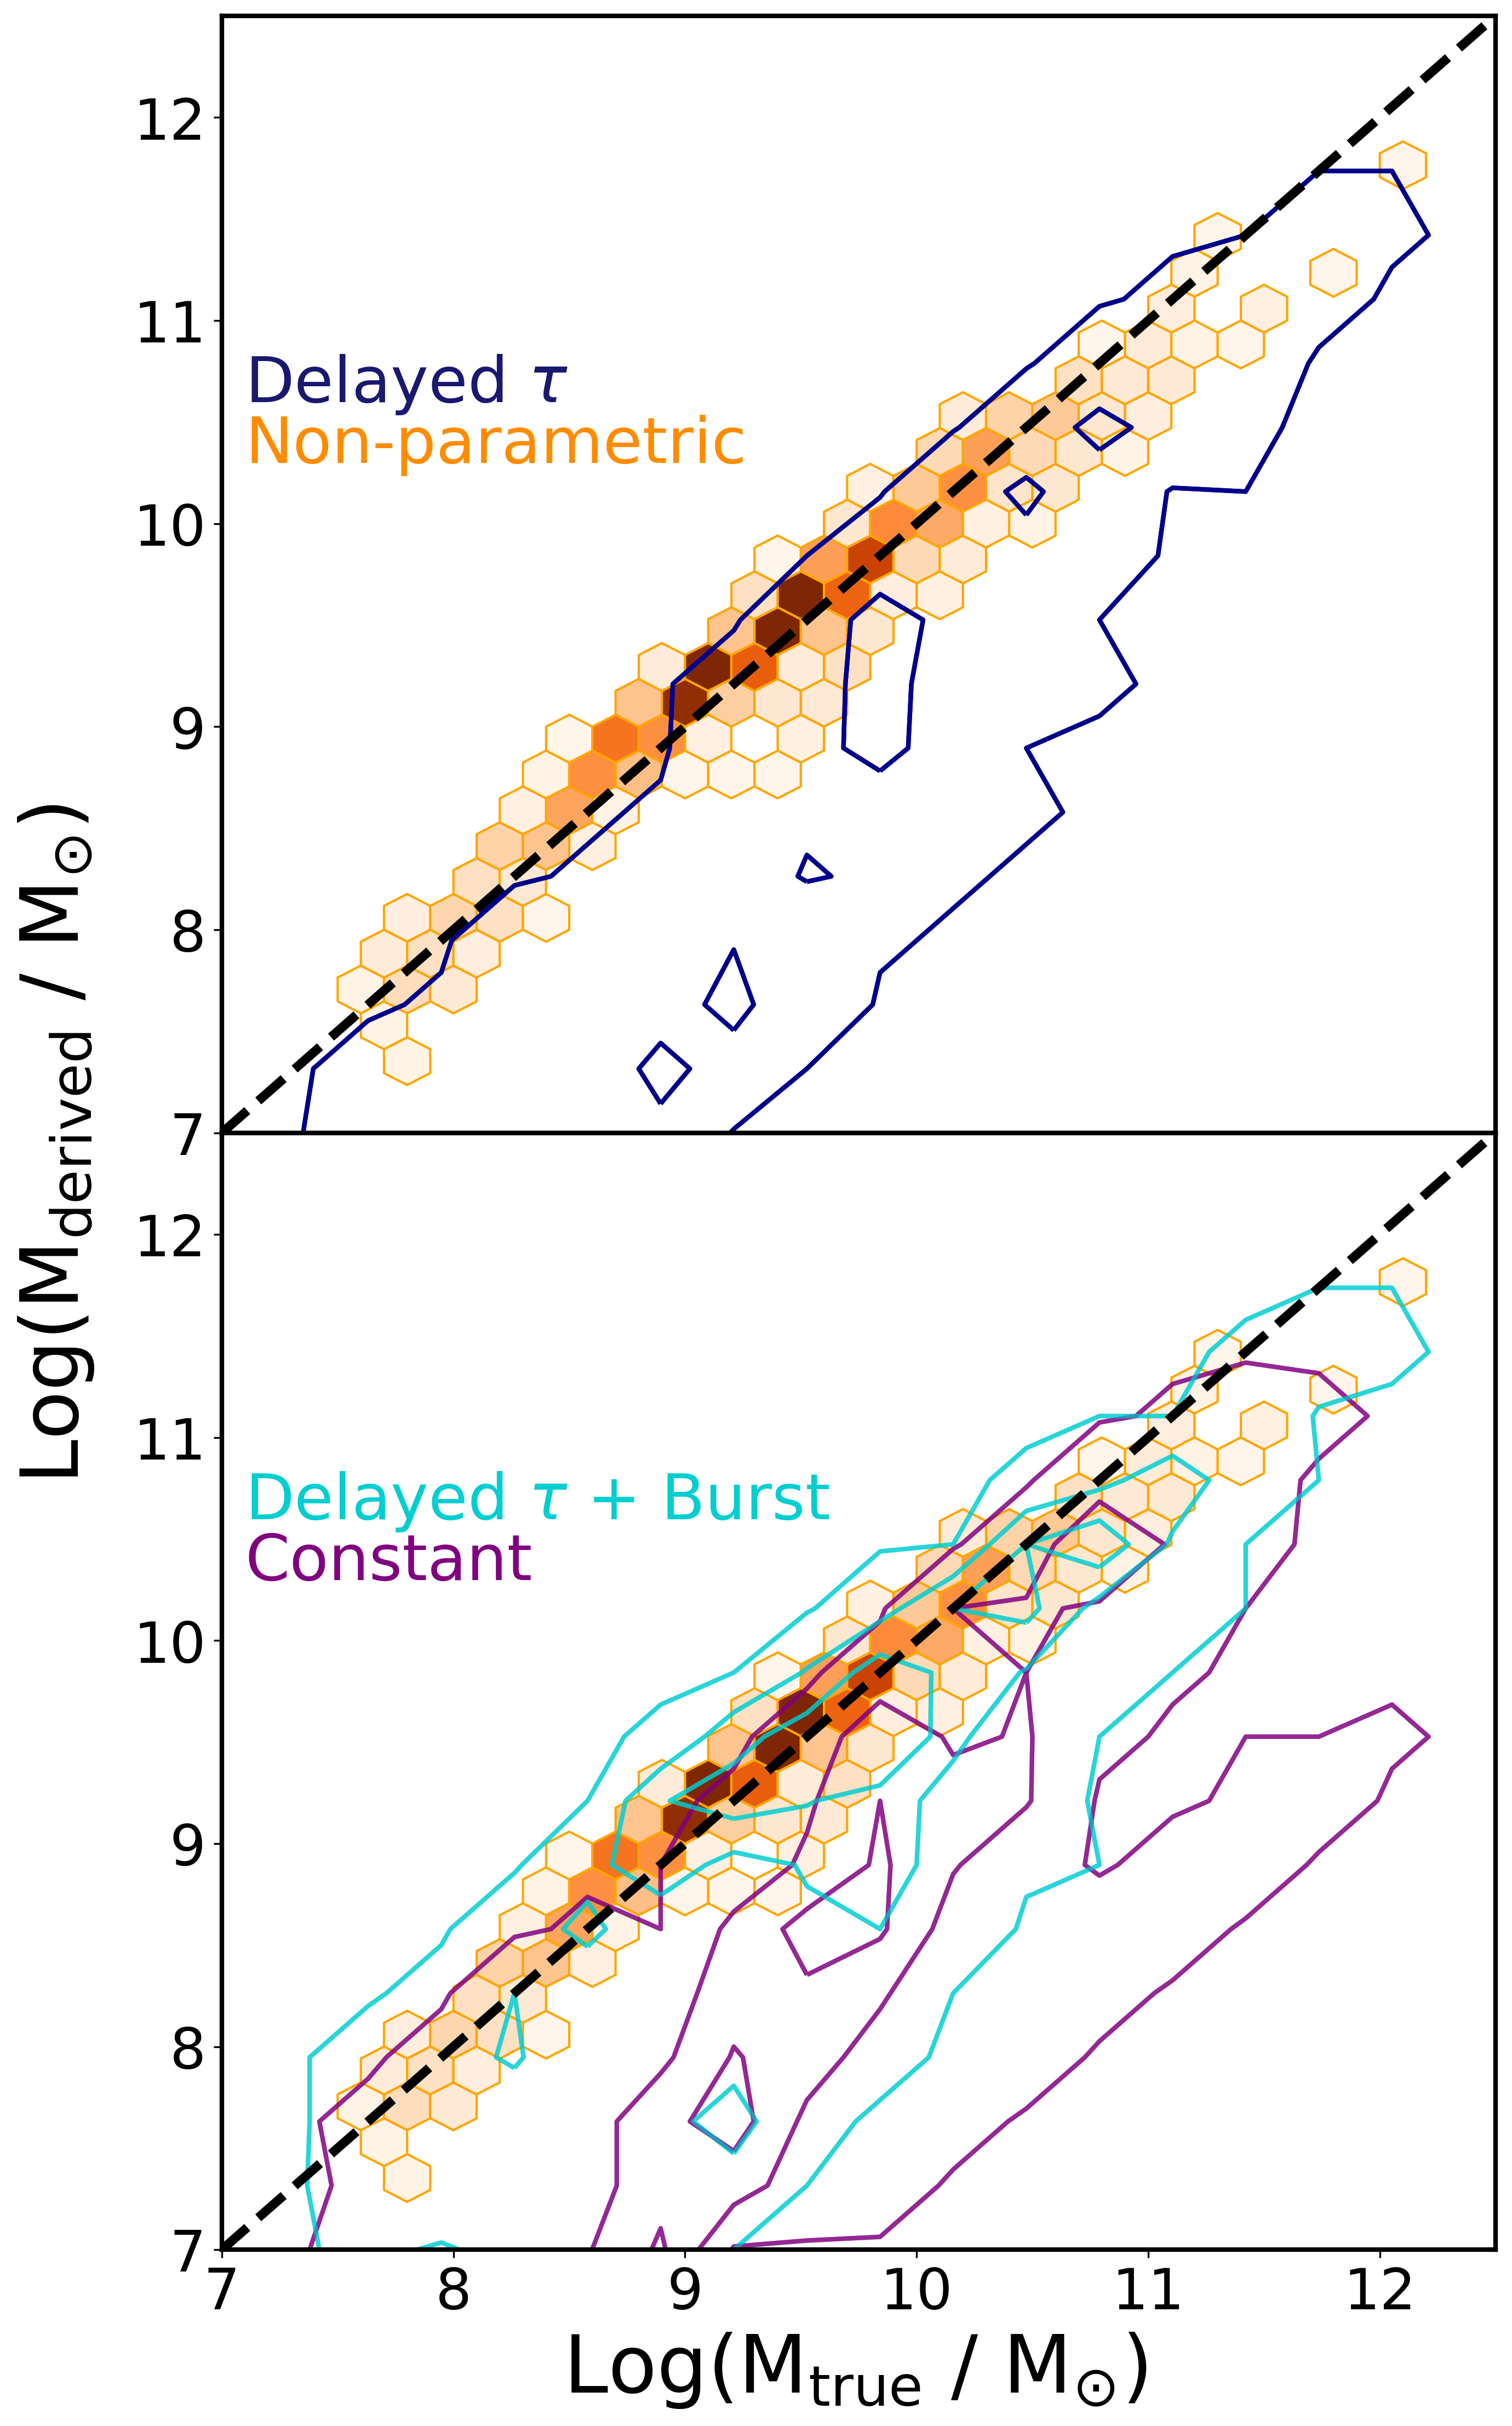
\includegraphics[width=0.41\textwidth]{mass_comp_sideways.png}}\hfill
  \subfloat[]{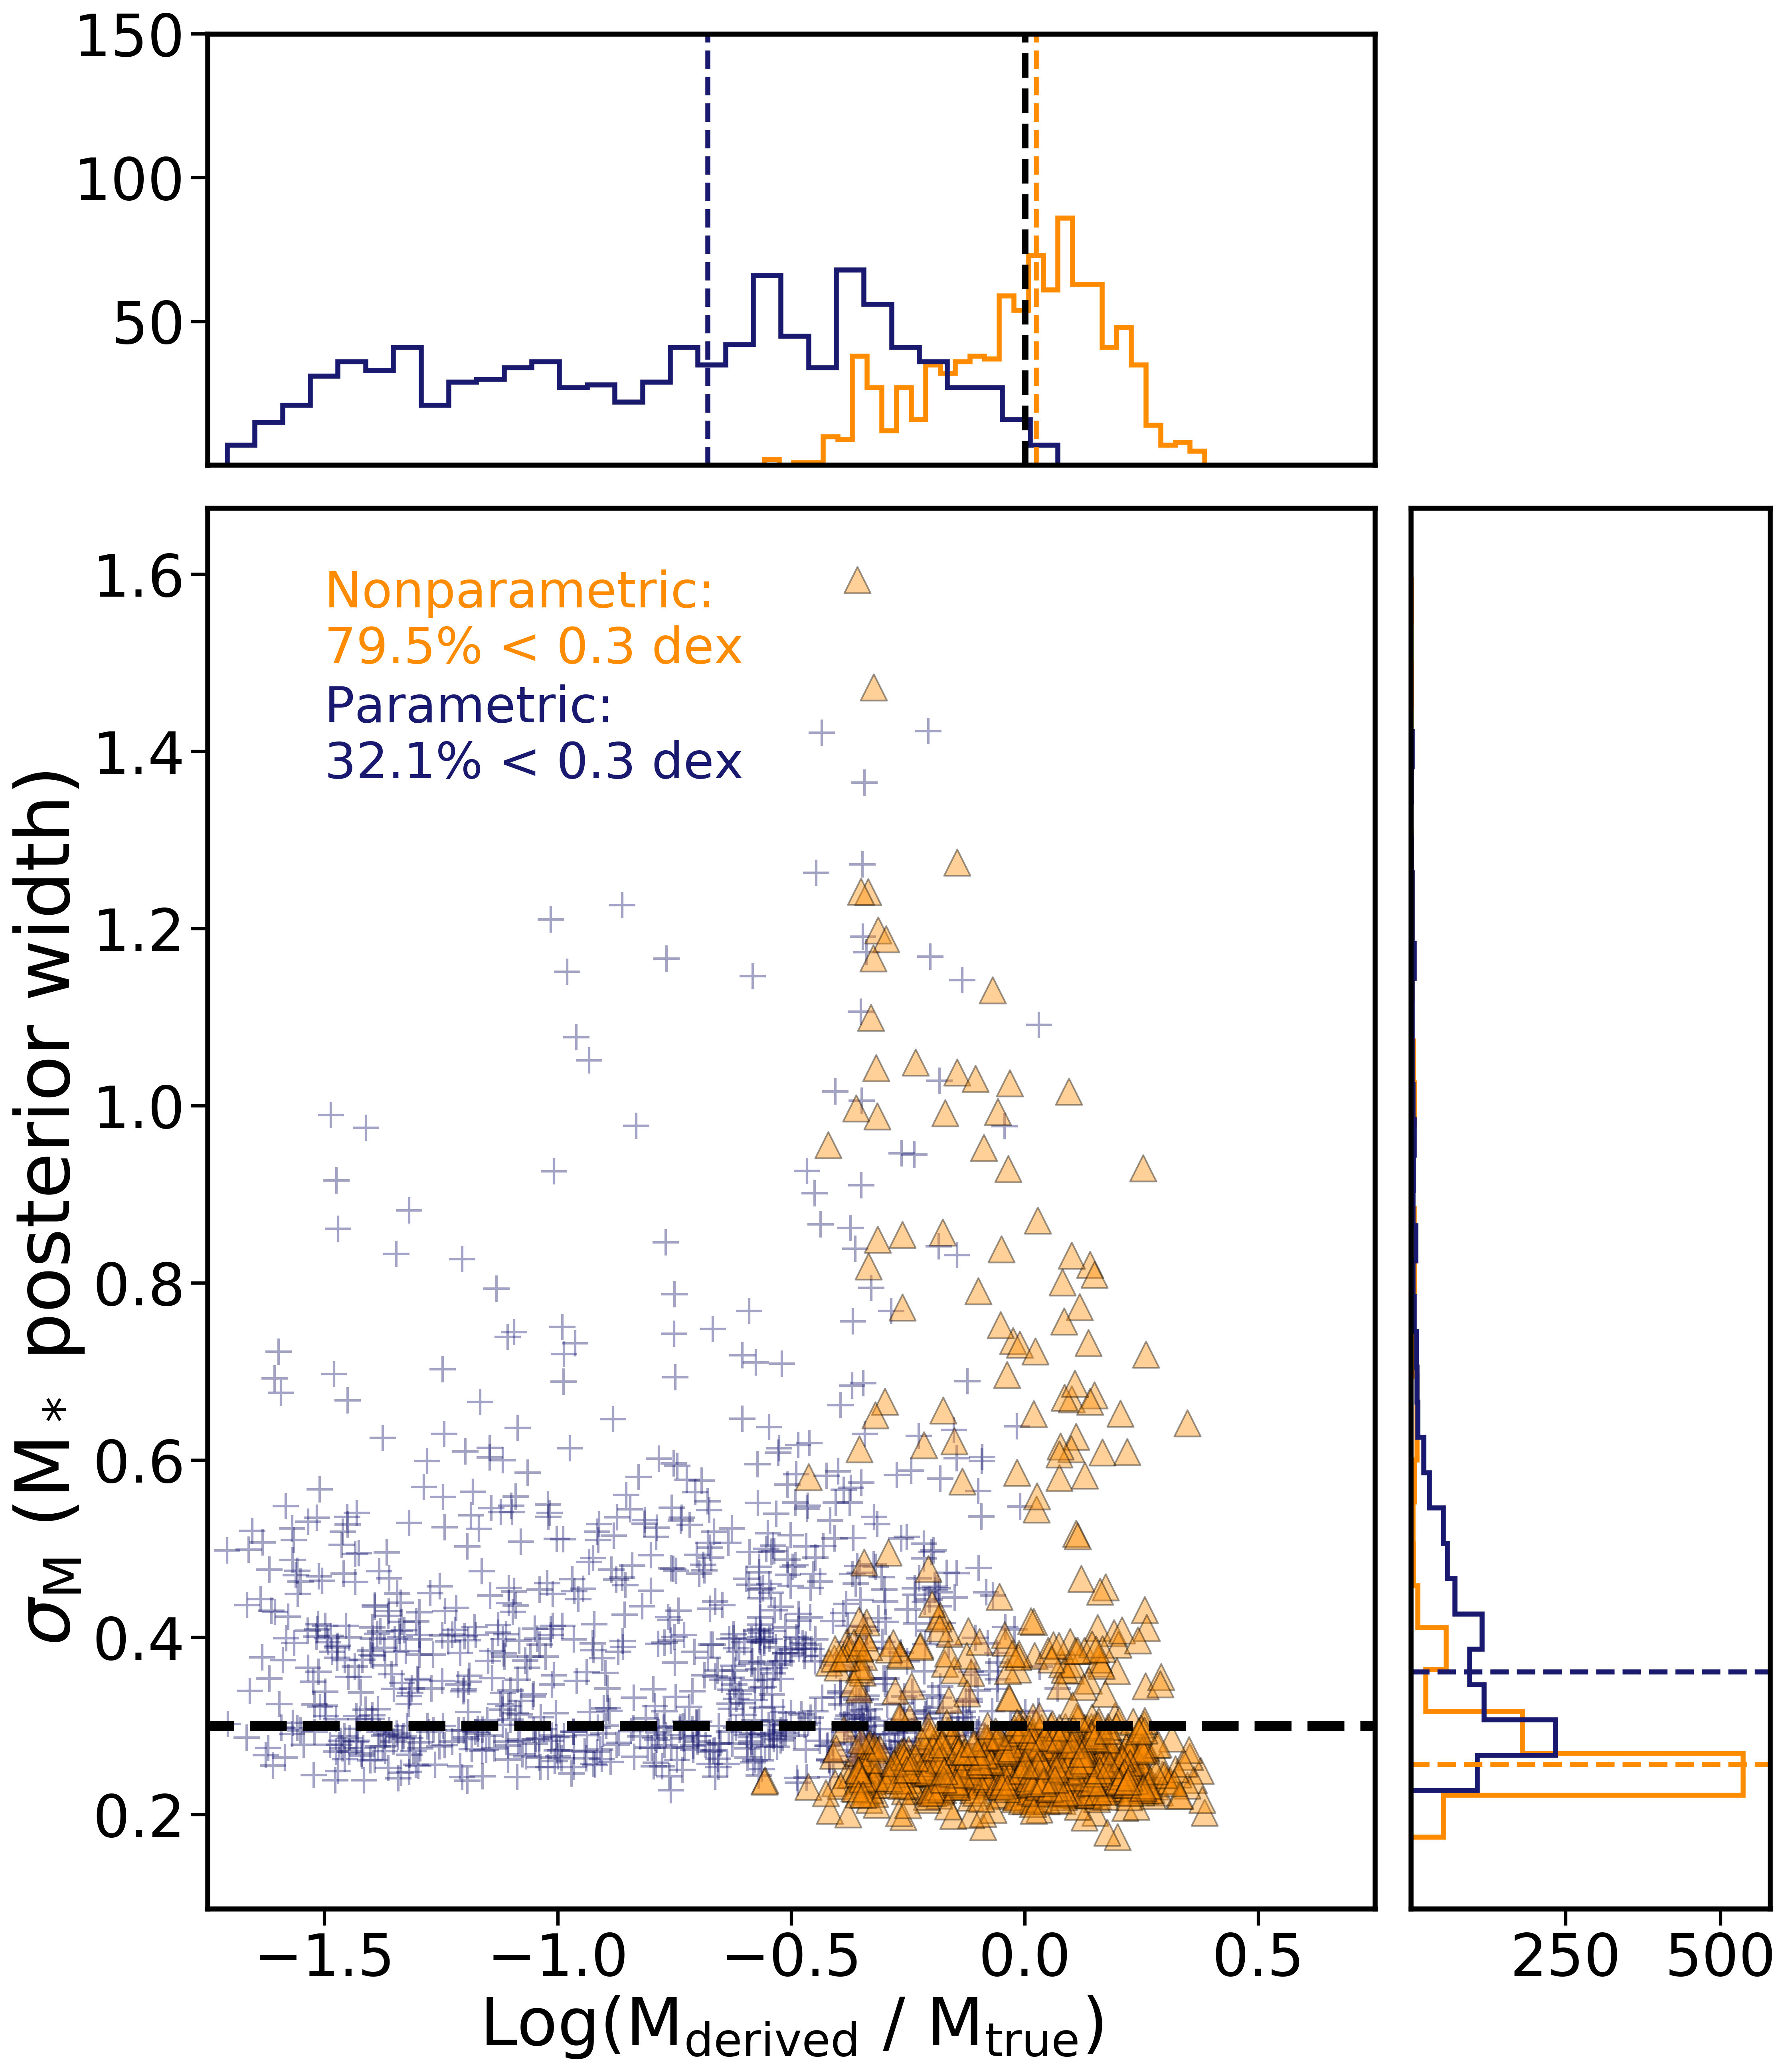
\includegraphics[width=0.56\textwidth]{Mscatter.png}}
  \caption{\textbf{Left}: Comparison of derived stellar masses to the true stellar masses of \texttt{simba} simulated galaxies for various SFH models. Top panel orange hexes represent stellar masses derived from the non-parametric SFH. Blue contours are stellar masses of the same galaxies this time derived from the delayed$-\tau$ SFH (a parametric model). Bottom panel is the same as left but purple contours show stellar masses derived using a constant SFH and turquoise contours show stellar masses derived using a delayed$-\tau$ with a burst component. \textbf{Right}: Uncertainty distribution of stellar mass estimates for a non-parametric model (orange) and a parametric (delayed$-\tau$) model (blue). The y-axis is the 1$-\sigma$ width of the estimated stellar mass posterior distributions for each galaxy. Histograms show the distribution of these points in log(M$_{\mathrm{ratio}}$) space and uncertainty space, where the colored dash lines show the median of each distribution. The percentage of masses that fall within 0.3 dex uncertainty ($\sim$factor of 2) for each SFH model is shown.}
\label{fig:mass_comp}
\end{figure*}

The primary objective of our analysis was understanding the underlying uncertainties in estimating M$_*$. Figure \ref{fig:mass_comp} shows the results for M$_*$. On the left is a comparison between the M$_*$ derived from the various SFH models described above. We compare the derived M$_*$ on the y-axis to the true M$_*$ on the x-axis. We see that the non-parametric models recover the true stellar masses with significantly better accuracy afforded by the flexibility of the SFH model. On the right shows the distribution in M$_*$ uncertainties for two of the SFH models, quantified as the 1$-\sigma$ widths of the Gaussian-like distributions. Close to 80\% of galaxies fit with a non-parametric form see uncertainties on M$_*$ below a factor of 2, a benchmark that many SED fitting codes and models therein have struggled to reach. Both plots show the significantly improved accuracy afforded by the non-parametric SFHs as compared to the traditional parametric forms. Though M$_*$ is considered the most robust property derived from SED fitting, the results here show a surprising reality: parametric SFHs fail for a majority of galaxies, across all stellar mass ranges. A more difficult impact to quantify is the affect of priors on the subsequent M$_*$ uncertainties. These priors are applied to the variables describing the features of a parametric SFH (e.g. $\tau$ in the delayed$-\tau$ form) and the derived physical properties from these SFH models are heavily dependent on the choice of prior distributions such that the priors tend to falsely narrow constraints resulting in under-estimated uncertainties. Thus, the distribution of uncertainties in Figure \ref{fig:mass_comp} for the parametric model may be too optimistic. 

\subsection{Star Formation History Recovery}\label{section:sfhs}

We also compare the best fit star formation histories to the true values. That the non-parametric star formation histories are more accurate at recovering the stellar mass of a galaxy is mainly attributed to the fact that they are much more flexible and thus better at describing the various star formation histories seen in the \texttt{simba} simulation. With only a small number of parameters describing the width and location of the curve, the three parametric SFHs (delayed-$\tau$, delayed-$\tau$ with a burst component, and constant), struggle to match the true SFH for most galaxies. This will affect not only the estimated stellar mass but also the derived stellar ages. The two delayed-$\tau$ models struggle to match the true SFHs that rise over time, as only very large values of $\tau$ allow for a slower decline at late times. For massive galaxies (M$_*$ $>$ $10^{11} \mathrm{M_{\odot}}$) at redshift z=0, the exponentially declining nature of these SFHs tends to match true galaxy SFHs better as these massive galaxies have dimished star formation or have stopped forming stars entirely. The lower mass galaxies tend to be bluer, star forming galaxies with SFHs ill-suited for the exponential decline at late times, so that the SFHs are not weel recovered and the stellar mass estimates will be worse, a point confirmed by Figure \ref{fig:mass_comp}.

\begin{figure}[h]

\centering
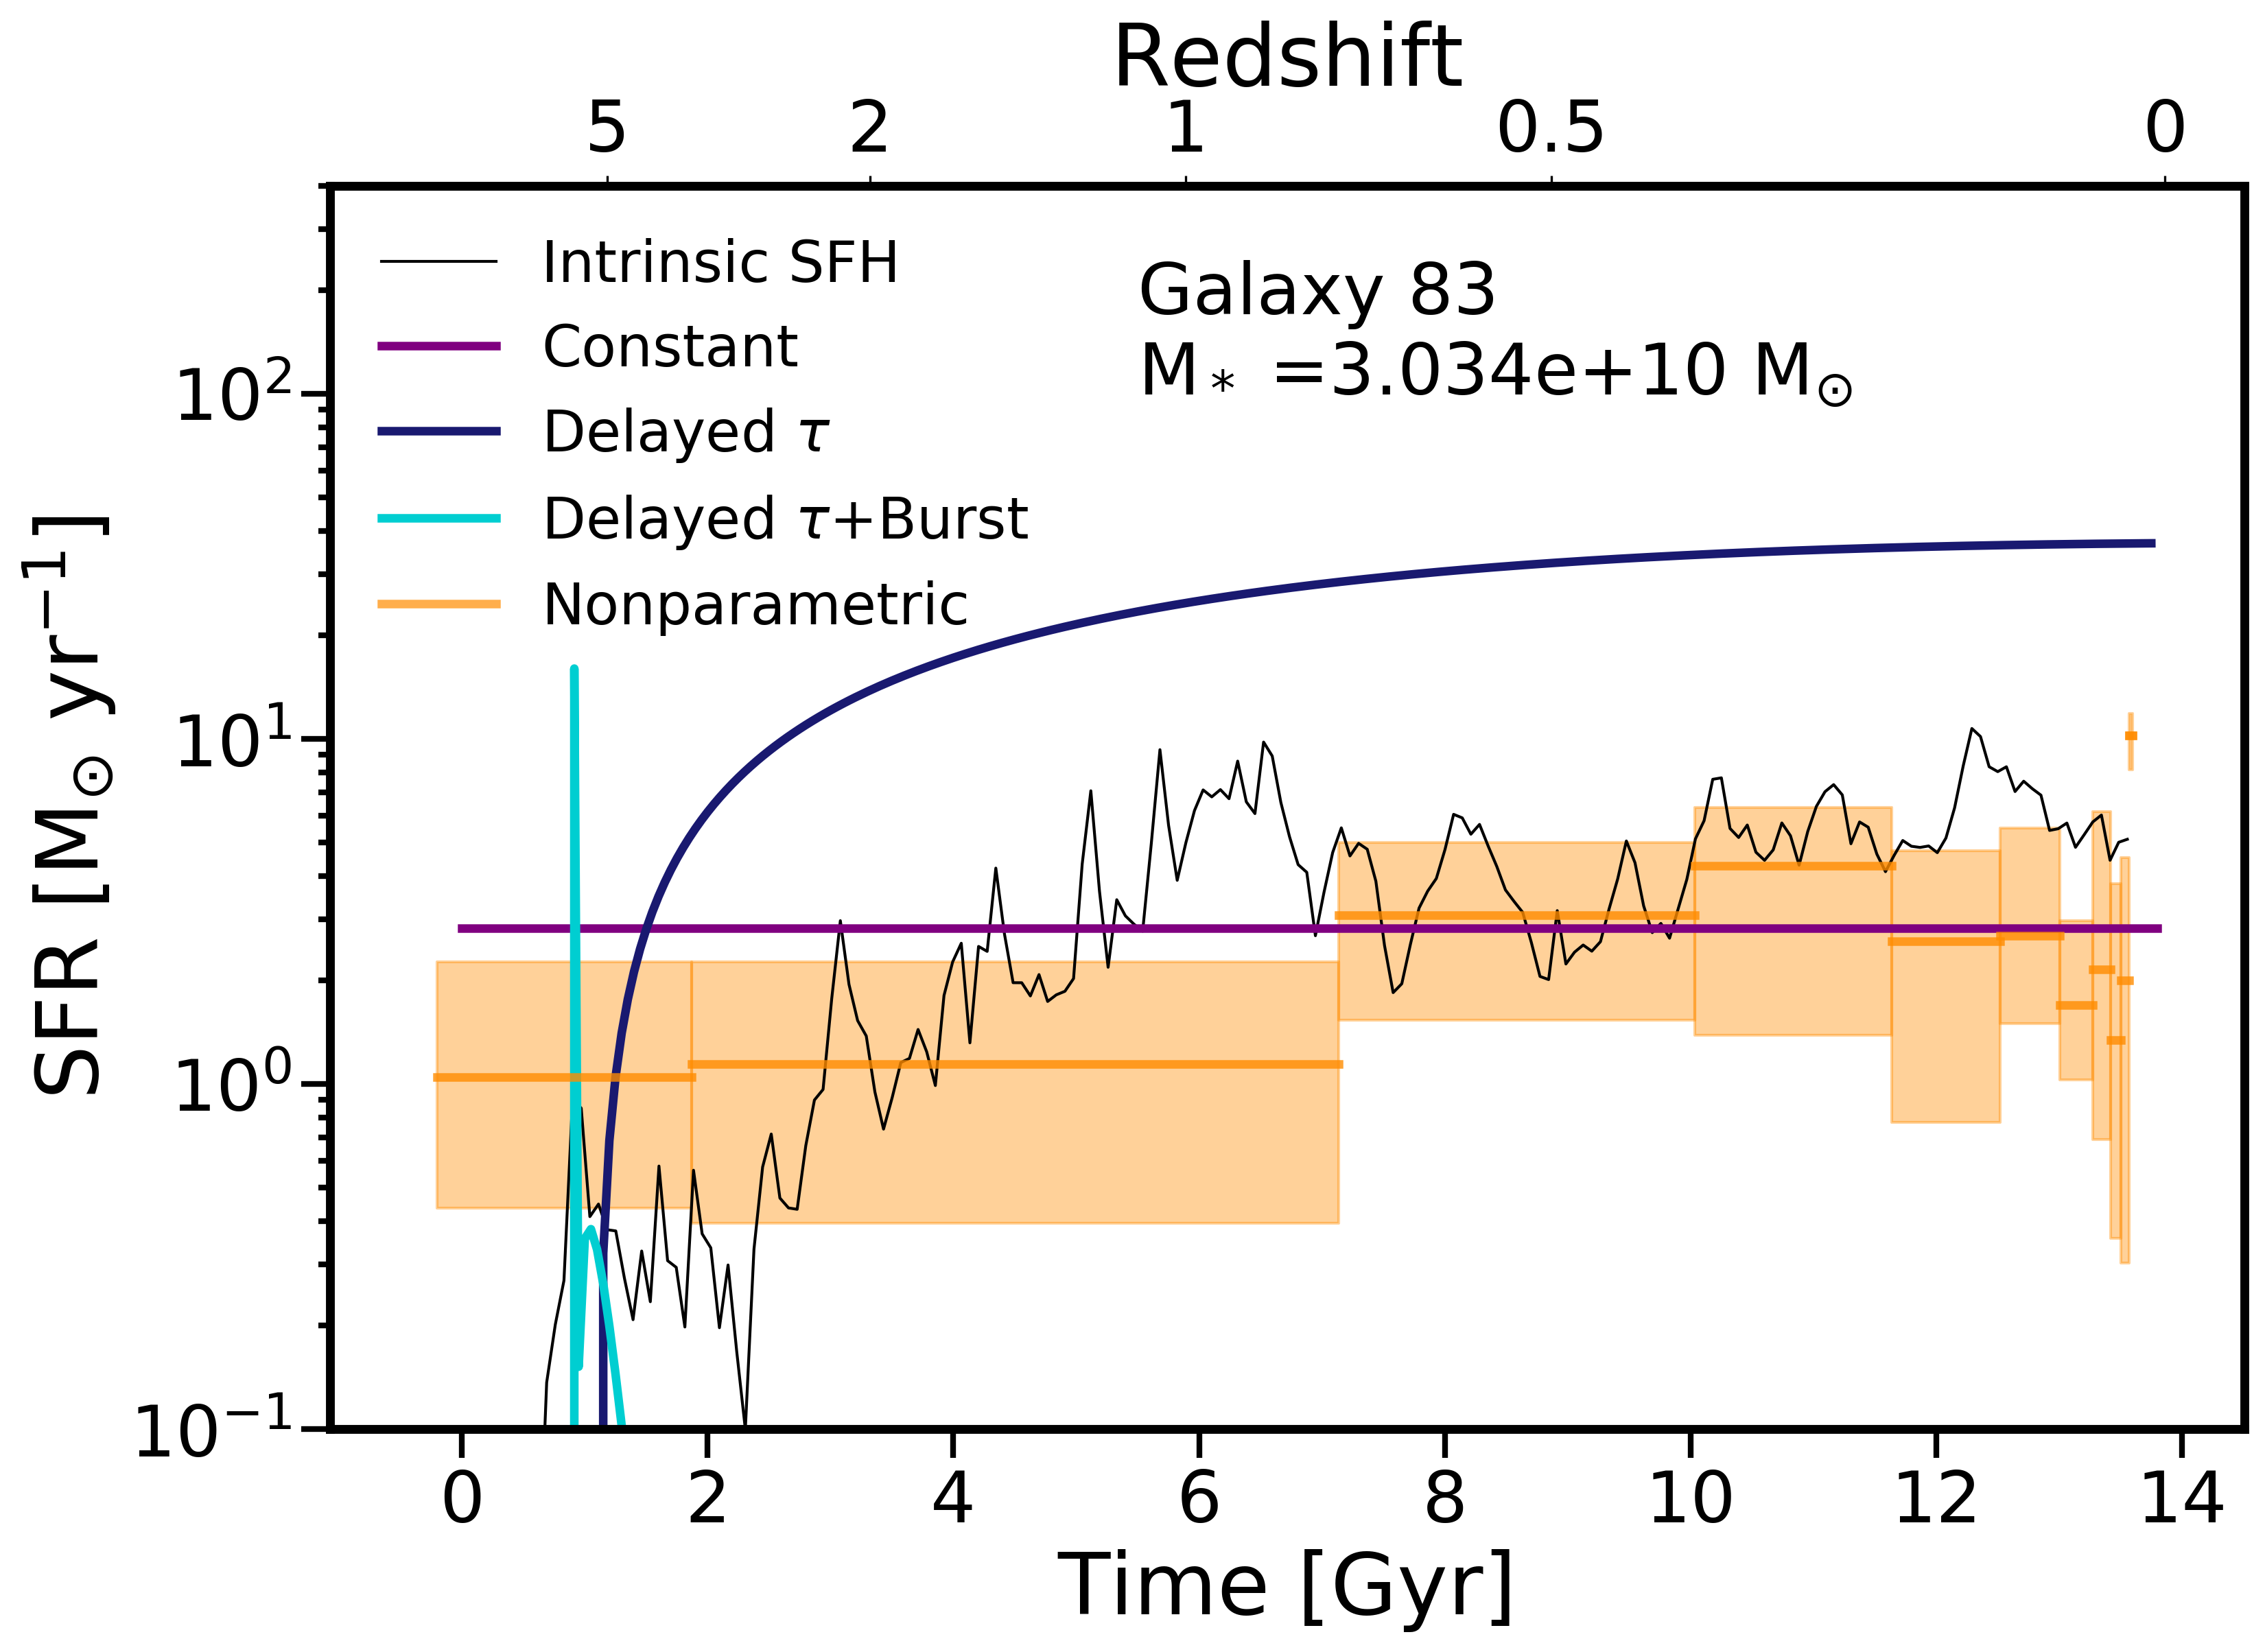
\includegraphics[width=0.47\textwidth]{SFH_83.png}
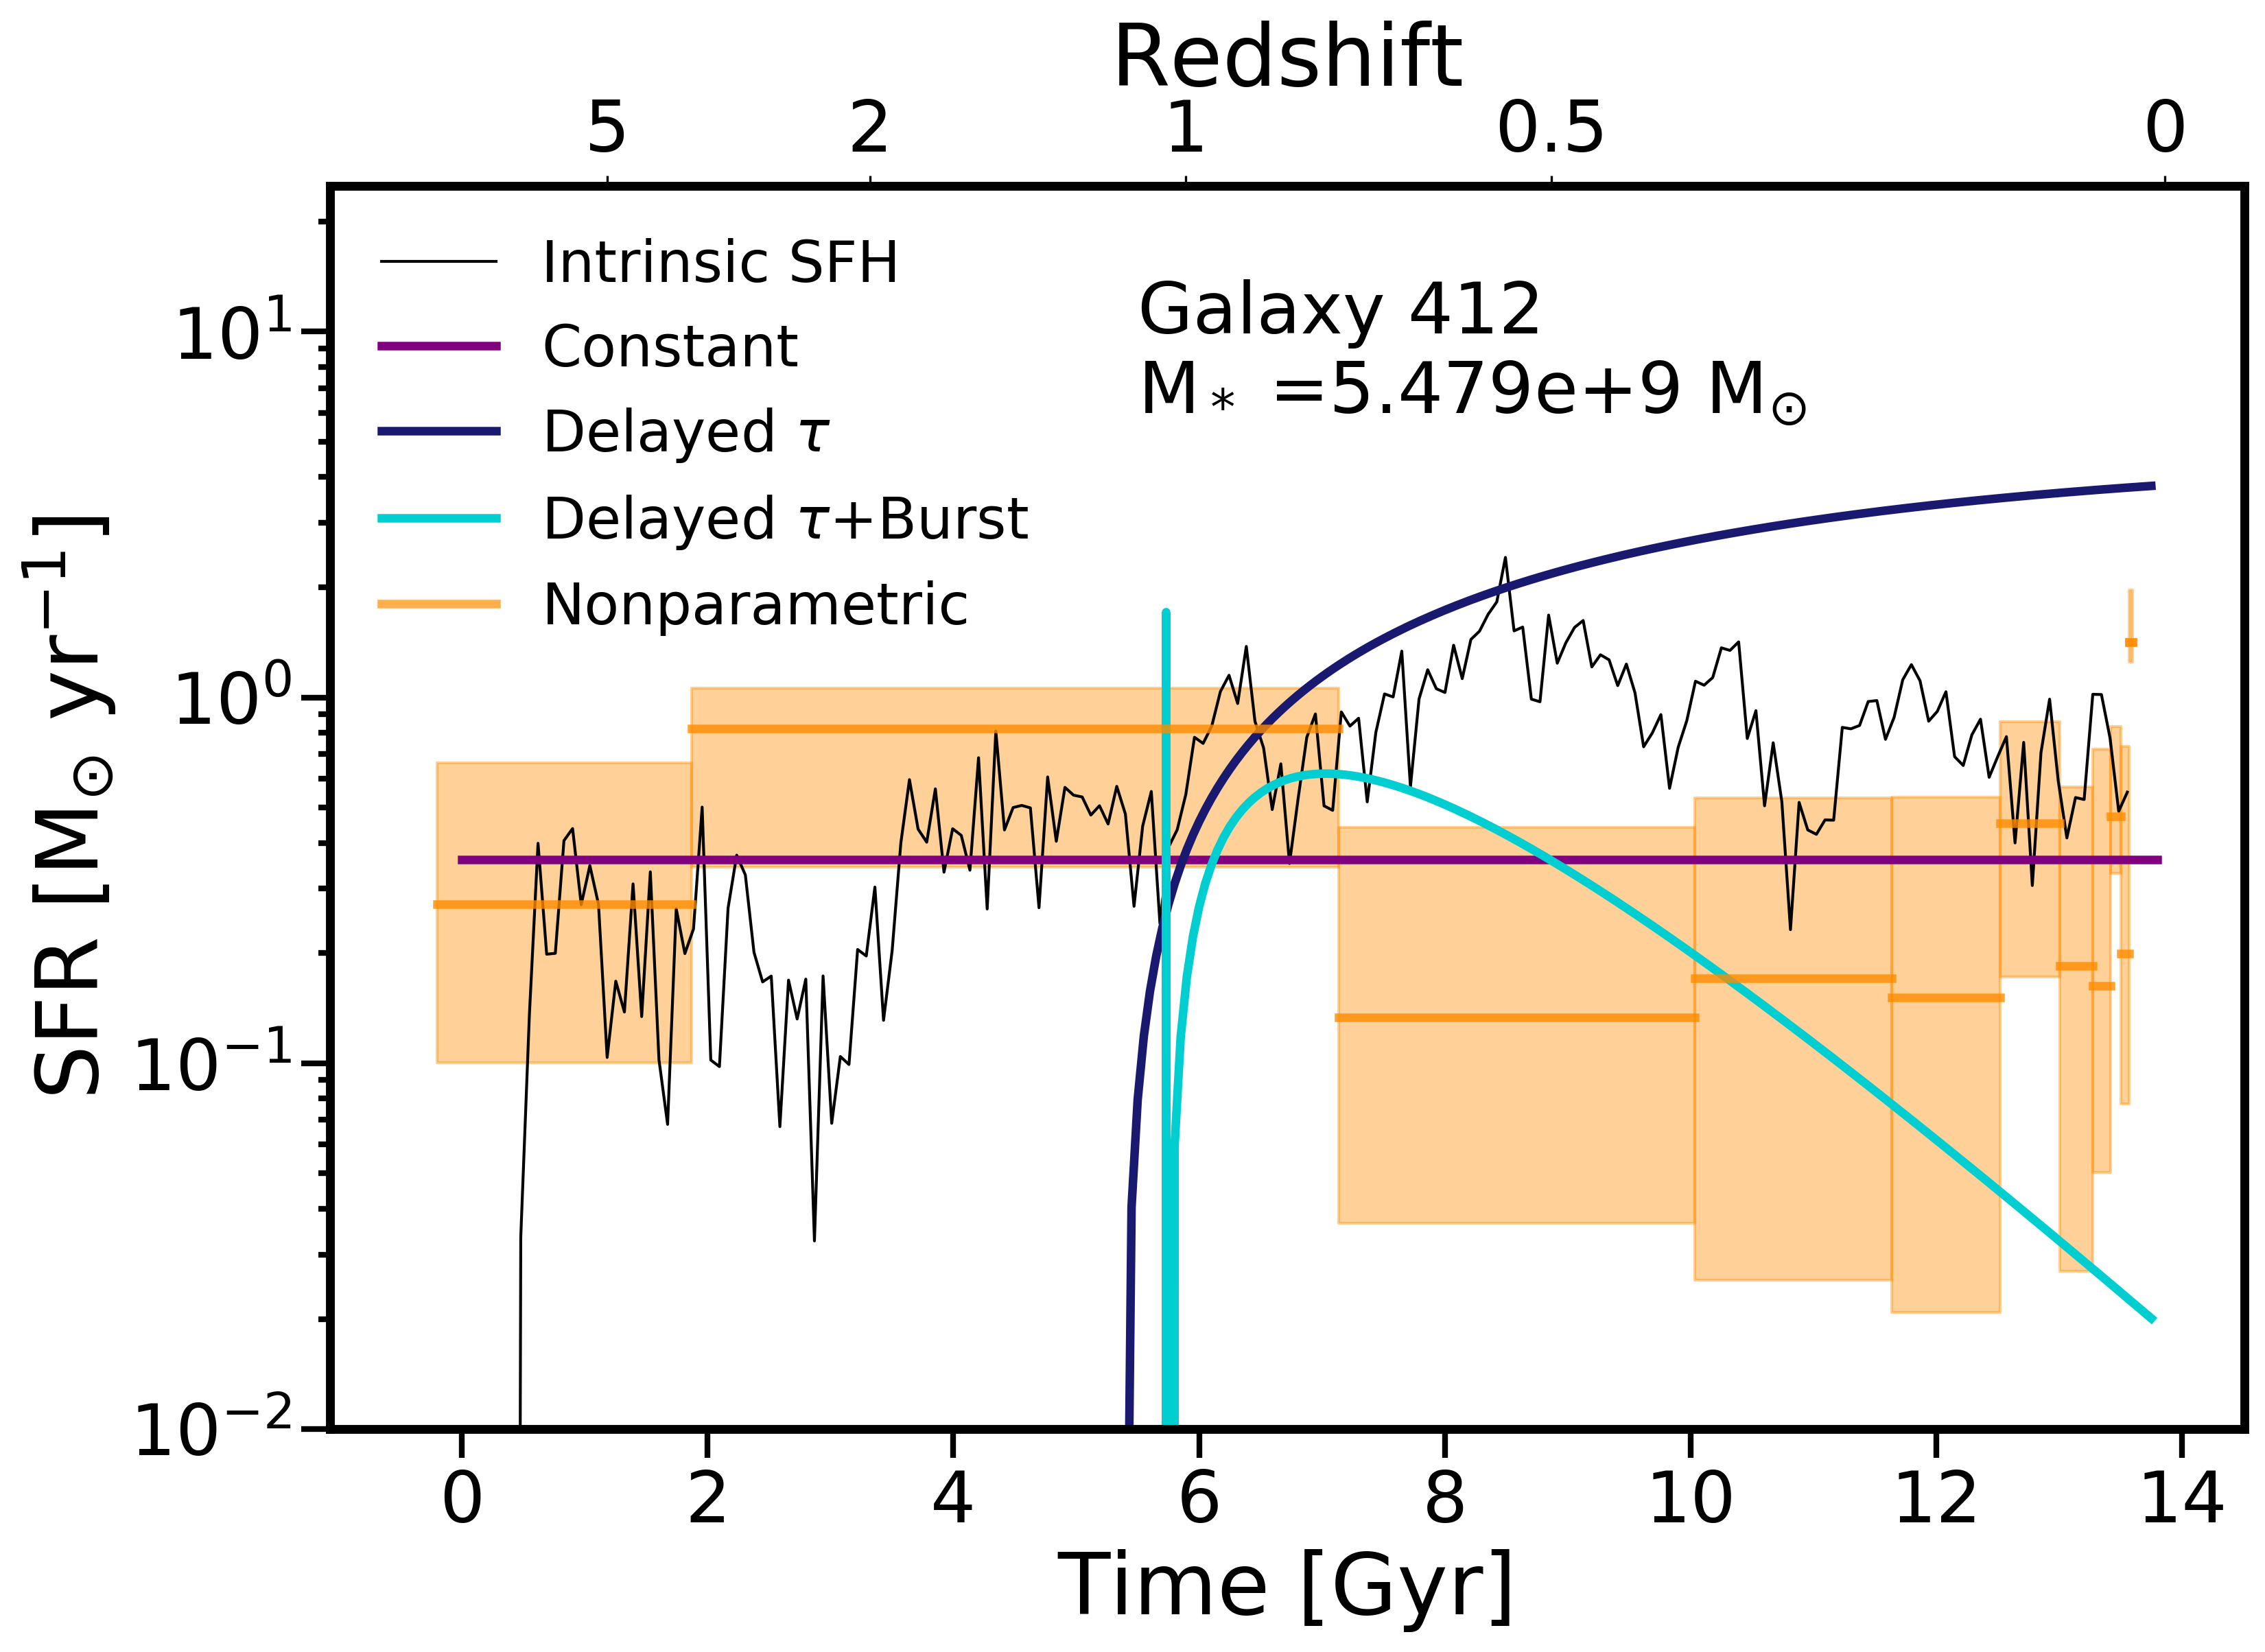
\includegraphics[width=0.47\textwidth]{SFH_412.png}

\caption{Star formation history for two example galaxies. The true galaxy SFH is shown in black. The fitted parametric forms are shown in dark blue (delayed-$\tau$), turquoise (delayed-$\tau$ plus burst), and purple (constant). The fitted non-parametric model is shown in orange. The $50^{\mathrm{th}}$ percentile value is shown as the solid line for the non-parametric SFH while the shaded regions include the $16^{\mathrm{th}}$ through $84^{\mathrm{th}}$ percentiles.}
\label{fig:sfh}

\end{figure}

Figure \ref{fig:sfh} shows two randomly chosen galaxy SFHs, comparing the recovered best-fit SFH for each model. The solid lines for each model refer to the median SFH while the shaded region encloses the 16th$-$84th percentiles for the non-parametric model (the 1$-\sigma$ region is neglected for the parametric models for clarity). The non-parametric SFHs shown here are comprised of 11 time bins separated logarithmically in time, except for the last two bins spanning the previous 10 Myr and 10$-$30 Myr, allowing for a minimally young population of stars. Though the derived stellar mass from these SFHs depends on the choice of timebins, we considered multiple iterations of bin numbers and durations and saw little changes in uncertainties past N $\gtrapprox$ 6 for this level of photometric coverage and uncertainty. By far the largest uncertainties and mismatches in derived physical properties occurred due to using a parametric SFH and not due to prior choices in the non-parametric model components.  



\subsection{Ages and Star Formation Rates}\label{section:ages}

Aside from M$_*$ and the recovered SFH, the estimated stellar ages and recent star formation rates provide further diagnostics into the power of non-parametric star formation histories, as recovering the true star formation history of a galaxy requires accurately estimating both the stellar mass and age of the stars formed. Figure \ref{fig:age_sfr} shows two histograms showing the distribution of estimated stellar ages and star formation rates over the last 10 Myr. Again, the non-parametric model shows marked improvement over the various parametric models in recovering the correct mass-weighted stellar ages. Parametric models, especially the delayed-$\tau$ form, struggle to match the correct age, with the estimated mass-weighted ages biased towards higher values.

\begin{figure}[h]

\centering
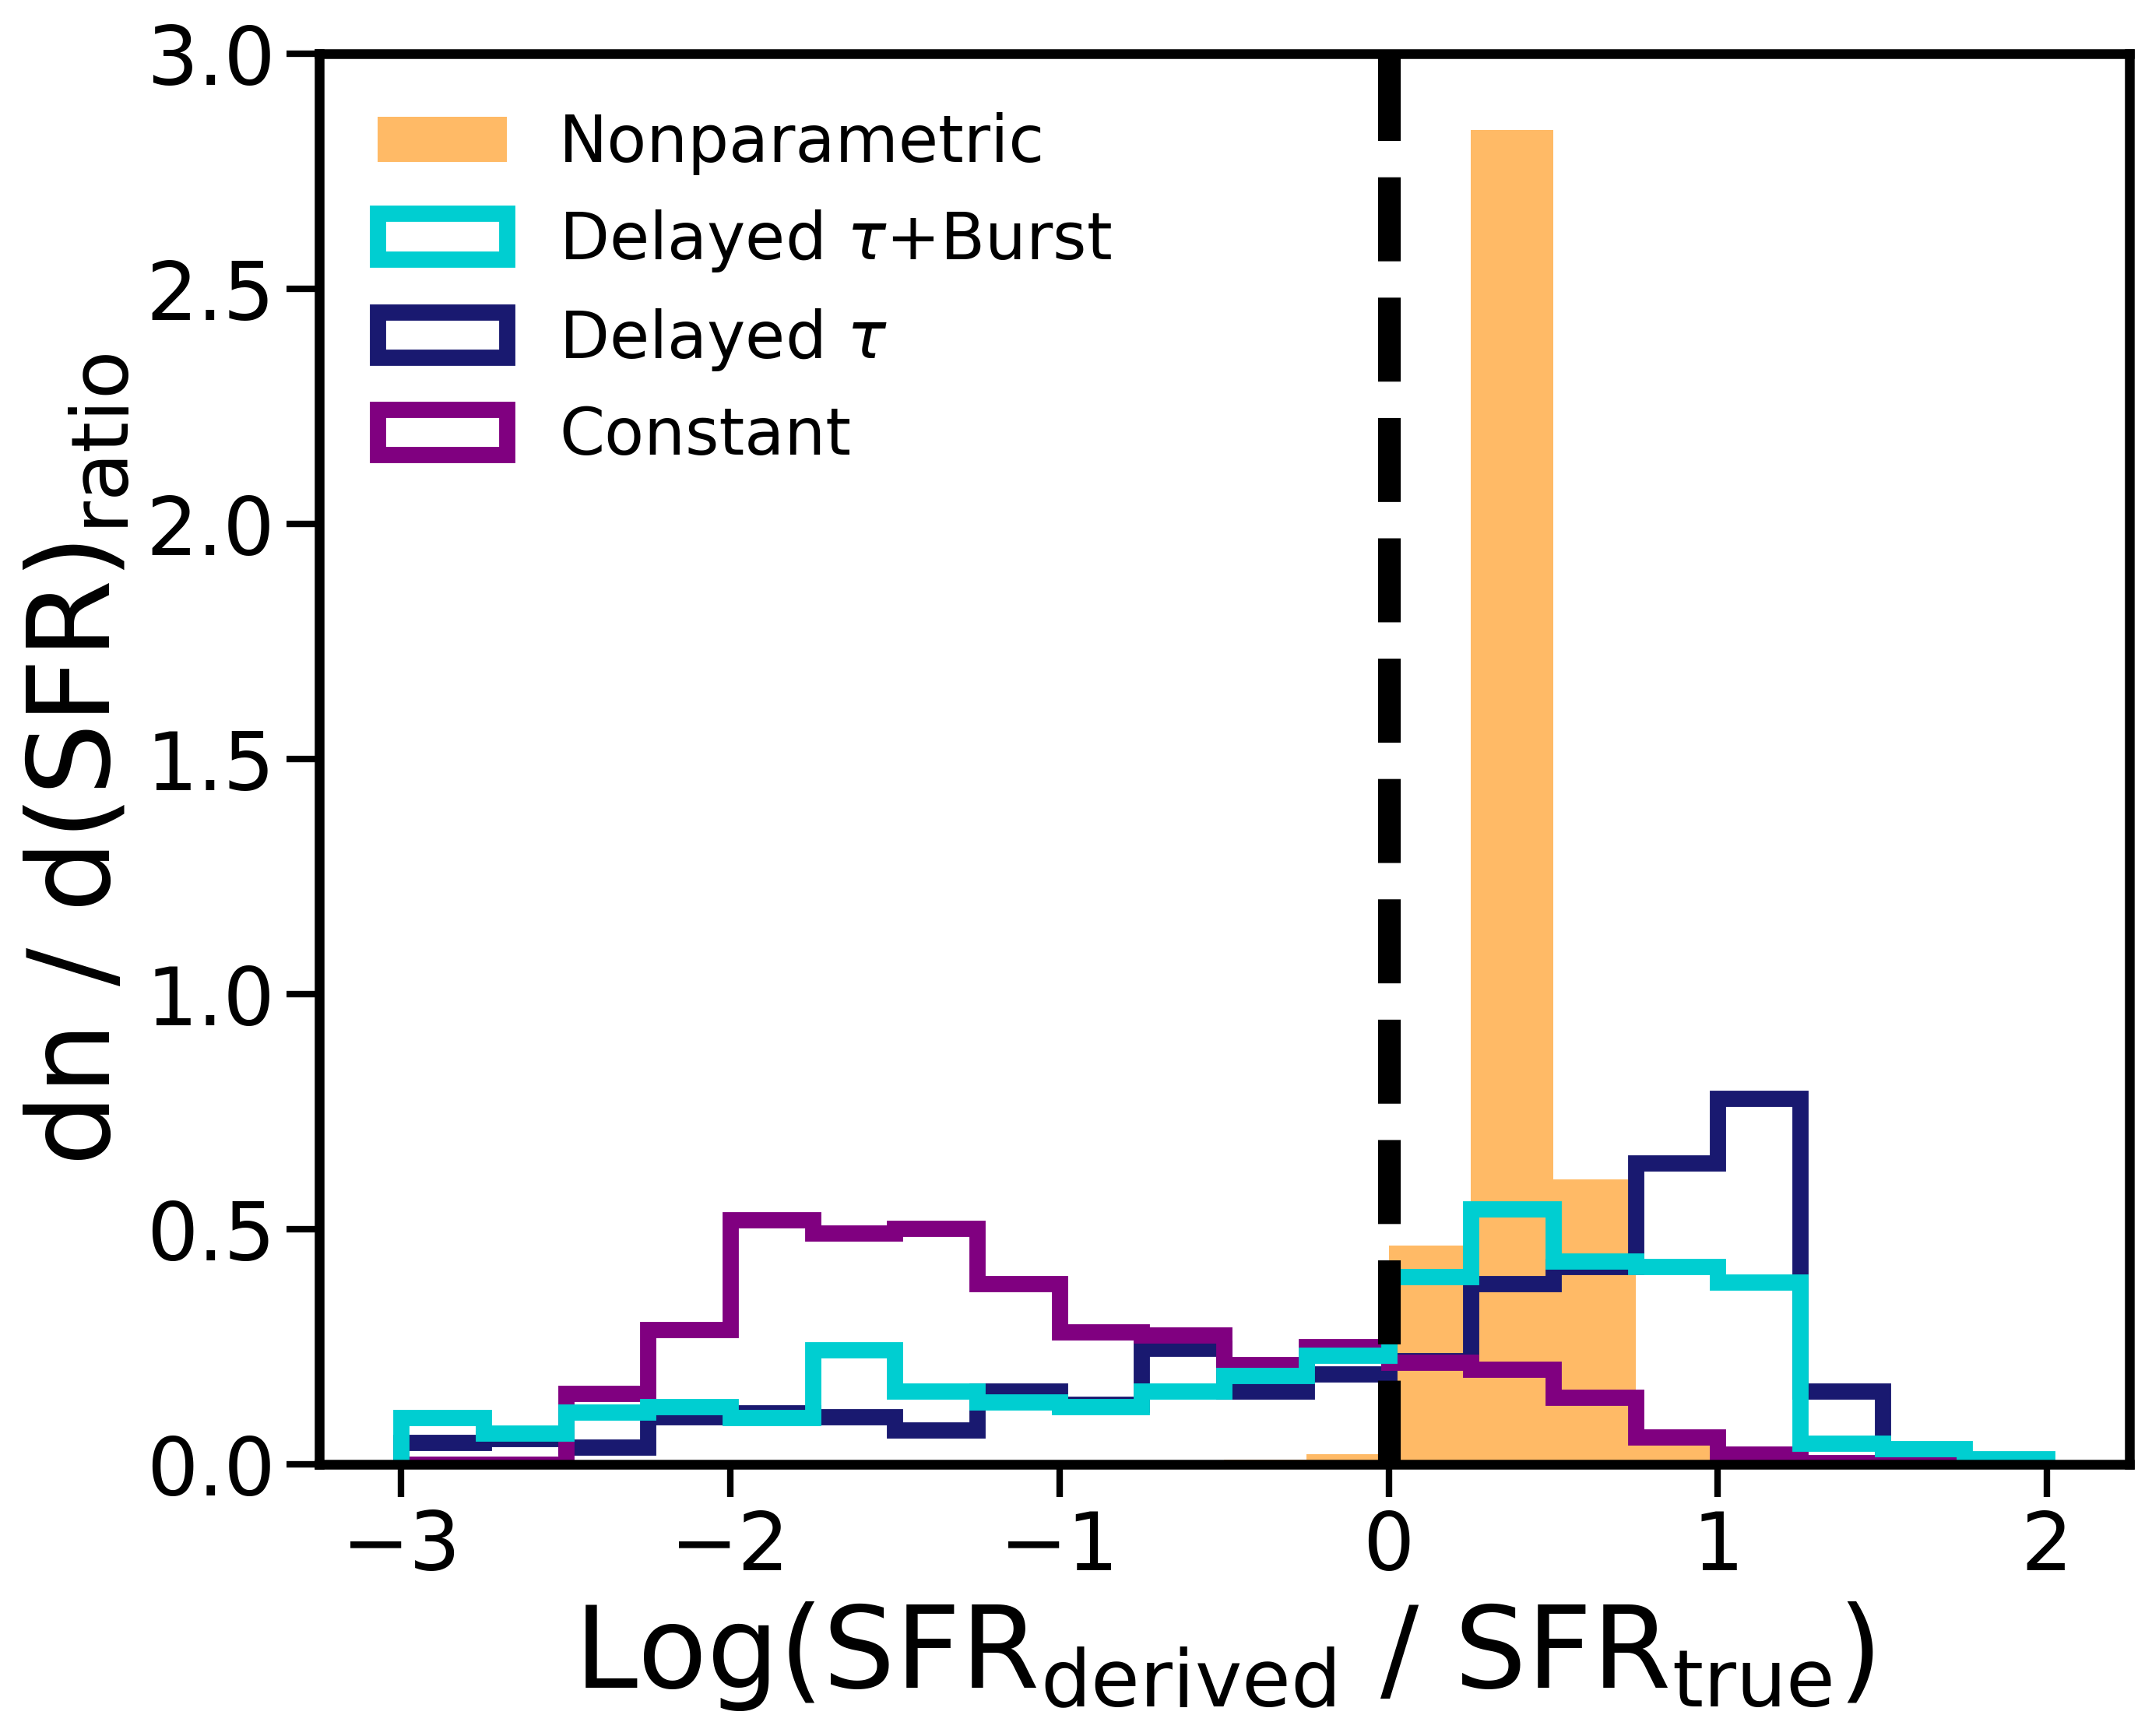
\includegraphics[width=0.47\textwidth]{SFRhist_all.png}\hfill
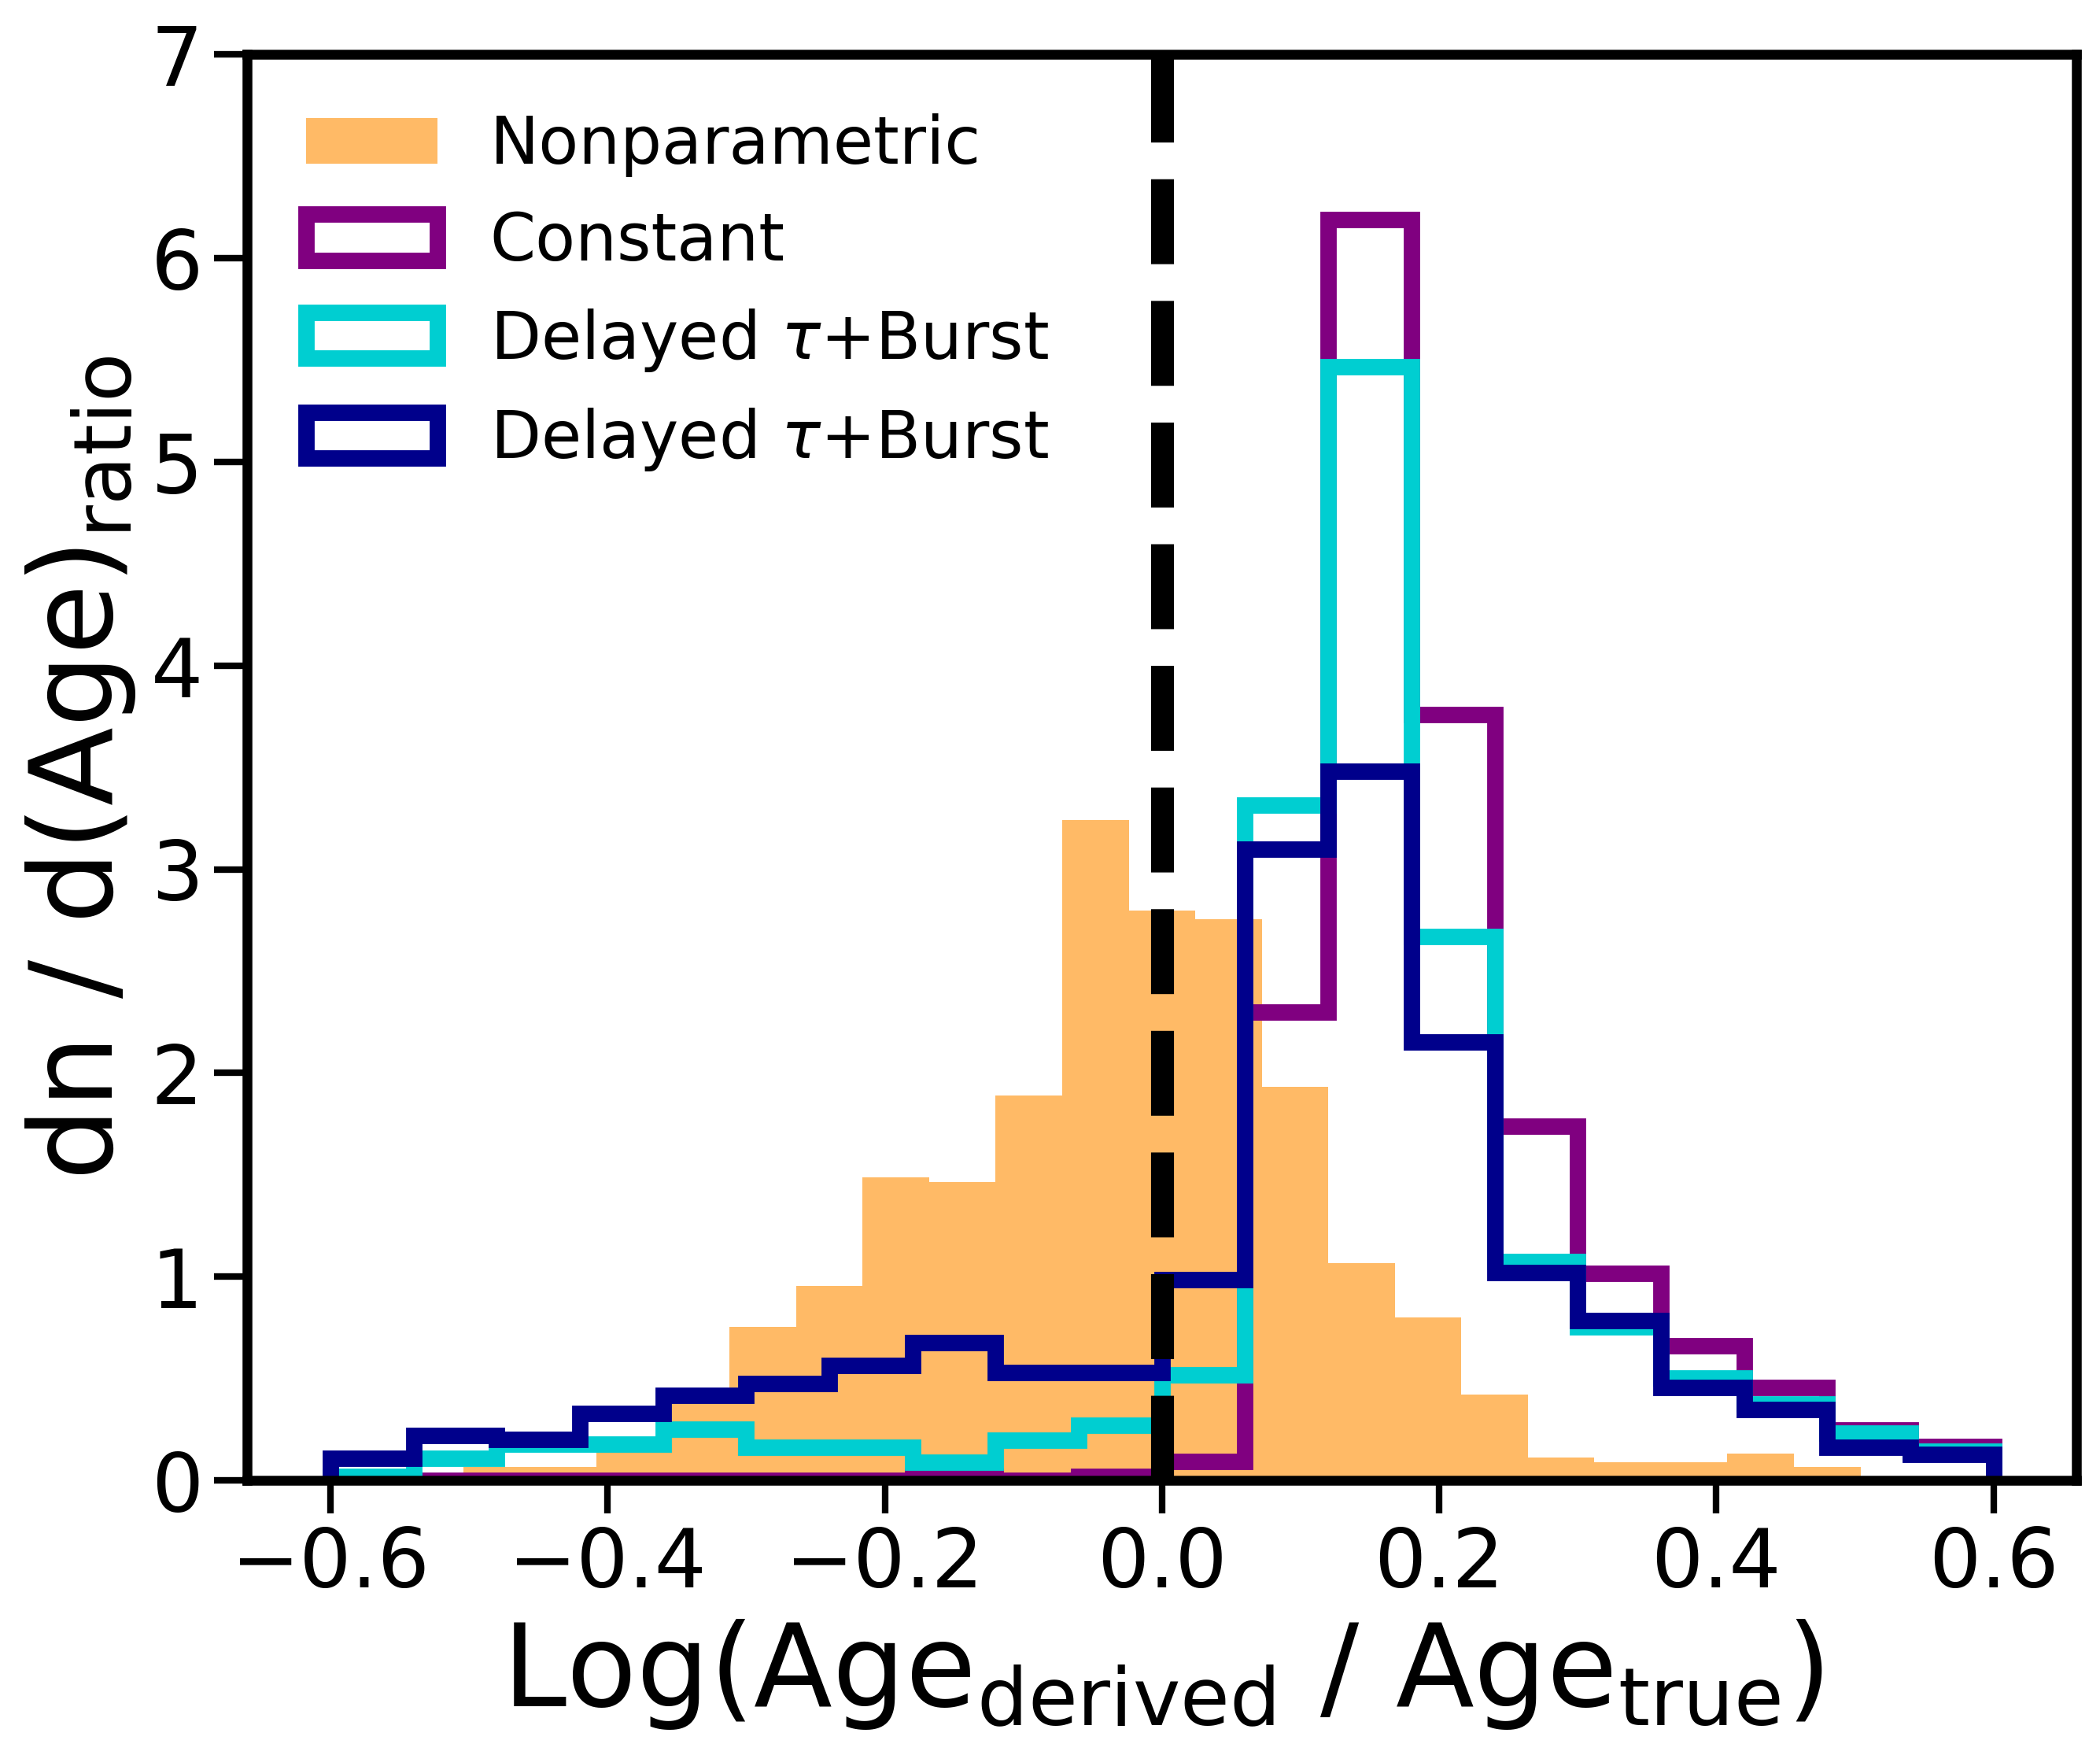
\includegraphics[width=.47\textwidth]{Agehist_taubdir.png}

\caption{\textbf{Top}: The distribution of the ratio of \texttt{prospector} derived star formation rates to the true star formation rates taken over the last 10 Myr. The black dashed line shows a 1:1 relation. The distributions for the three parametric SFHs extend to $\mathrm{log(SFR}_{\mathrm{derived}} / \mathrm{SFR}_{\mathrm{true}}$) = -10. \textbf{Bottom}: The ratio of \texttt{prospector} derived mass-weighted stellar ages to the true stellar ages.}
\label{fig:age_sfr}

\end{figure}

However, as shown in Figure \ref{fig:age_sfr}, the non-parametric SFH systematically overestimates the late time star formation rate of galaxies. The SFR over the last 10 Myr represents the most recent bin of star formation (i.e. it is the 11$^{th}$ out of the 11 bins of star formation that were varied in the SED fit). The probable cause of the bias seen in SFR$_{10 \: \mathrm{Myr}}$ is discussed in \ref{section:fail}, where we explore various origins of the discrepancies in stellar mass estimates. Even so, it is clear the delayed-$\tau$ parametric forms also fail to recover the late time star formation rate. This is due to the nature of the exponential declining SFH, biasing SFR$_{10 \mathrm{Myr}}$ to lower values. Removing this prior, as in the case of the non-parametric SFH, allows the late time behavior to not necessarily be tied to another epoch of star formation. This greater flexibility allows for more accurate stellar ages, SFHs, and stellar masses. 


\section{Discussion}

On average, the non-parametric SFHs outperform the parametric SFHs in all metrics, including estimating M$_*$ and accurately recovering the mass-weighted stellar ages and late time star formation rate. At the minor expense of computation time, the more flexible SFHs are able to more accurately reconstruct the physical properties and growth history of galaxies. The improved accuracy is owed to the greater flexibility of the non-parametric models. A by-eye analysis of the library of star formation histories measured from the \texttt{simba} simulation show that the $\tau$ and delayed-$\tau$ SFH models are a poor match for a majority of the galaxy population at redshift z=0. Moreover, the danger in blindly applying a delayed-$\tau$ SFH to a sample of galaxies lies in the false constraints on galaxy properties imposed by the SFH priors. This results in under-estimated uncertainties on the derived physical properties. Because the non-parametric forms do not impose such severe priors, the model uncertainties reflect the true uncertainties more accurately. 


\subsection{Applications: recovering observed star forming main sequence}\label{section:MS}

\begin{figure*}[t]

\centering
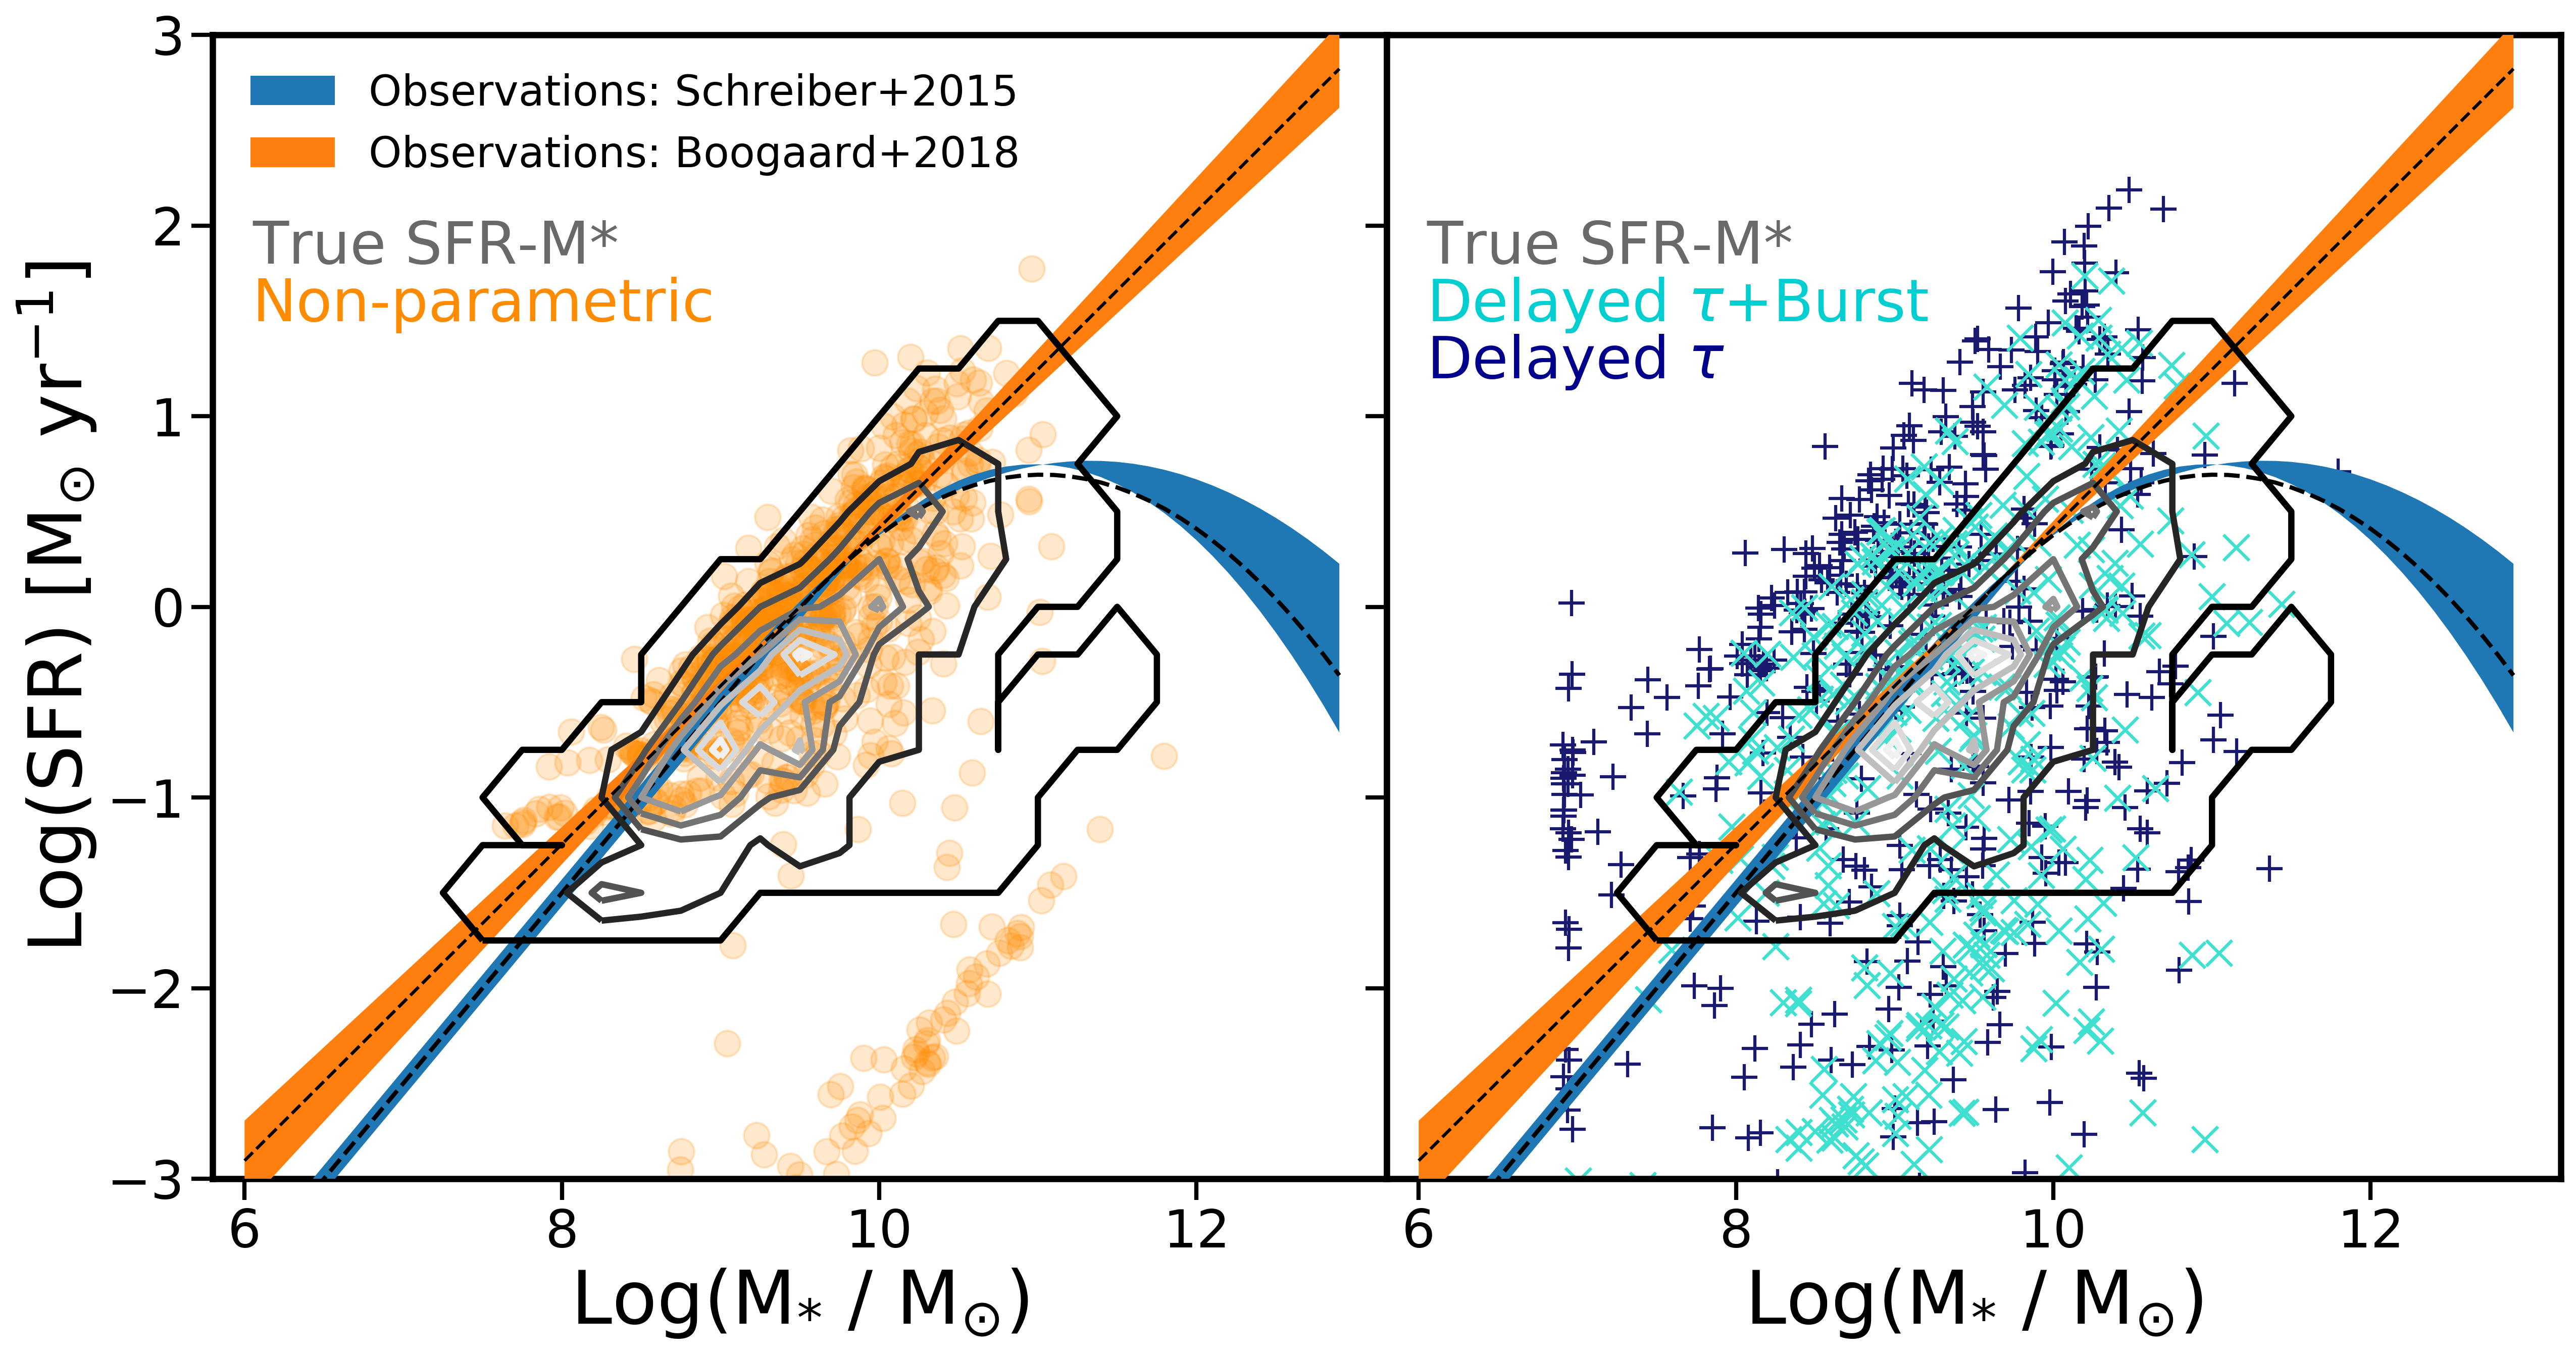
\includegraphics[width=\textwidth]{MS_twopanel.png}\hfill

\caption{The star forming main sequence as estimated from \texttt{prospector}, relating a galaxy's star formation thus far (stellar mass) to the current rate of star formation. Star formation rates are averaged over the last 100 Myr of the star formation history. Modeled values from SED fitting (scatter points) are compared to the true values from the simulation and to two curves from the literature (\cite{schreiber_herschel_2015}; \cite{boogaard_muse_2018}). \textbf{Left}: Values estimated from the non-parametric form are seen in orange. Intrinsic values are shown with gray contours. \textbf{Right}: Values estimated from the parametric forms are seen in the dark blue crosses (delayed-$\tau$), turquoise x's (delayed-$\tau$ plus burst) and purple diamonds (constant).}
\label{fig:sfms}
\end{figure*}

We now turn to understanding how the use of non-parameteric star formation histories in SED modeling can improve our understanding of classical scaling relations in galaxies.  We begin by understanding the location of our modeled galaxies on the star forming main sequence (SFMS).  In Figure \ref{fig:sfms}, we plot the star formation rate-stellar mass relation from our modeled galaxies {\it as they would be modeled observationally via SED modeling.}  That is, we do not plot the {\it true} SFR-$M_*$ relation as derived from the cosmological hydrodynamic simulations.  We use these models to compare to literature compilations by \citet{schreiber_herschel_2015} and \citet{boogaard_muse_2018}. The relation between these two properties is dependent on the ability of the SFH models to recover the correct SFH overall (and thus the stellar mass formed) and also the late time star formation rate over the last 10 Myr. Although from an observational point of view, the SFR is typically measured with star formation tracers (i.e. FIR luminosity, H$\alpha$ line flux) that each represent different physical time scales, the SFR averaged over the last 10 Myr of the SFH estimated by SED modeling is still a useful property. 

Due to the exponentially declining nature of the two parametric SFH models used here, the late time SFR estimated from these models tends to be much lower than the true value. On the other hand, the late time SFR estimated from the non-parametric SFHs tends to overestimate the true SFRs, as seen in Figure \ref{fig:sfms}. However, the scatter in SFR$_{10 \: \mathrm{Myr}}$ for the non-parametric models is much less than that of the parametric models. Synthesizing these two results, the non-parametric SFHs are able to recover both the intrinsic SFMS of galaxies and also match two observed relations from the literature (\cite{boogaard_muse_2018}, \cite{schreiber_herschel_2015}). 

\subsection{Where the SFH models fail}\label{section:fail}

Although on average the non-parametric SFH is more successful in recovering the intrinsic stellar masses of the \texttt{simba} galaxies, there are some galaxies whose estimated properties are catastrophic outliers from the ideal scenario of a 1:1 ratio between the true and derived property. As seen from the distribution in Figure \ref{fig:mass_comp}, the non-parametric SFH appears to struggle with the high mass end, but the lack of high mass galaxies (M$_*$ $>$ 10$^{11.5} \mathrm{M}_{\odot}$) in this specific \texttt{simba} box does not allow for statistically meaningful results to be gleaned from these failures. 

Wholesale conclusions are difficult to draw as to the reason why the SFH model fails, as the reasons are unique for each galaxy. Stellar age and star formation rate estimates serve as an further diagnostics on the performance of the non-parametric SFHs. For these properties, the scatter in the ratio of derived property to true value is again much smaller for the non-parametric models than the parametric models. Though we can see that the scatter tends to increase at the high mass end for both properties. Considering the degeneracy between the age of a galaxy and the level of dust attenuation, we could expect the older, more massive systems to suffer from greater uncertainty when estimating stellar masses. 

Intuitively, poor stellar mass and stellar age estimates originate from poor fits to the true galaxy SFH. The shape of the SFH will affect the stellar ages but the overall normalization will affect the prediction for the total stellar mass formed. Also intuitively, SFHs that are higher (lower) than the true SFH on average will predict stellar masses that are larger (smaller) than the true values. The question then becomes \textit{why did the non-parametric star formation histories fail to match the true values in some cases}? 

\begin{figure}[h!]

\centering
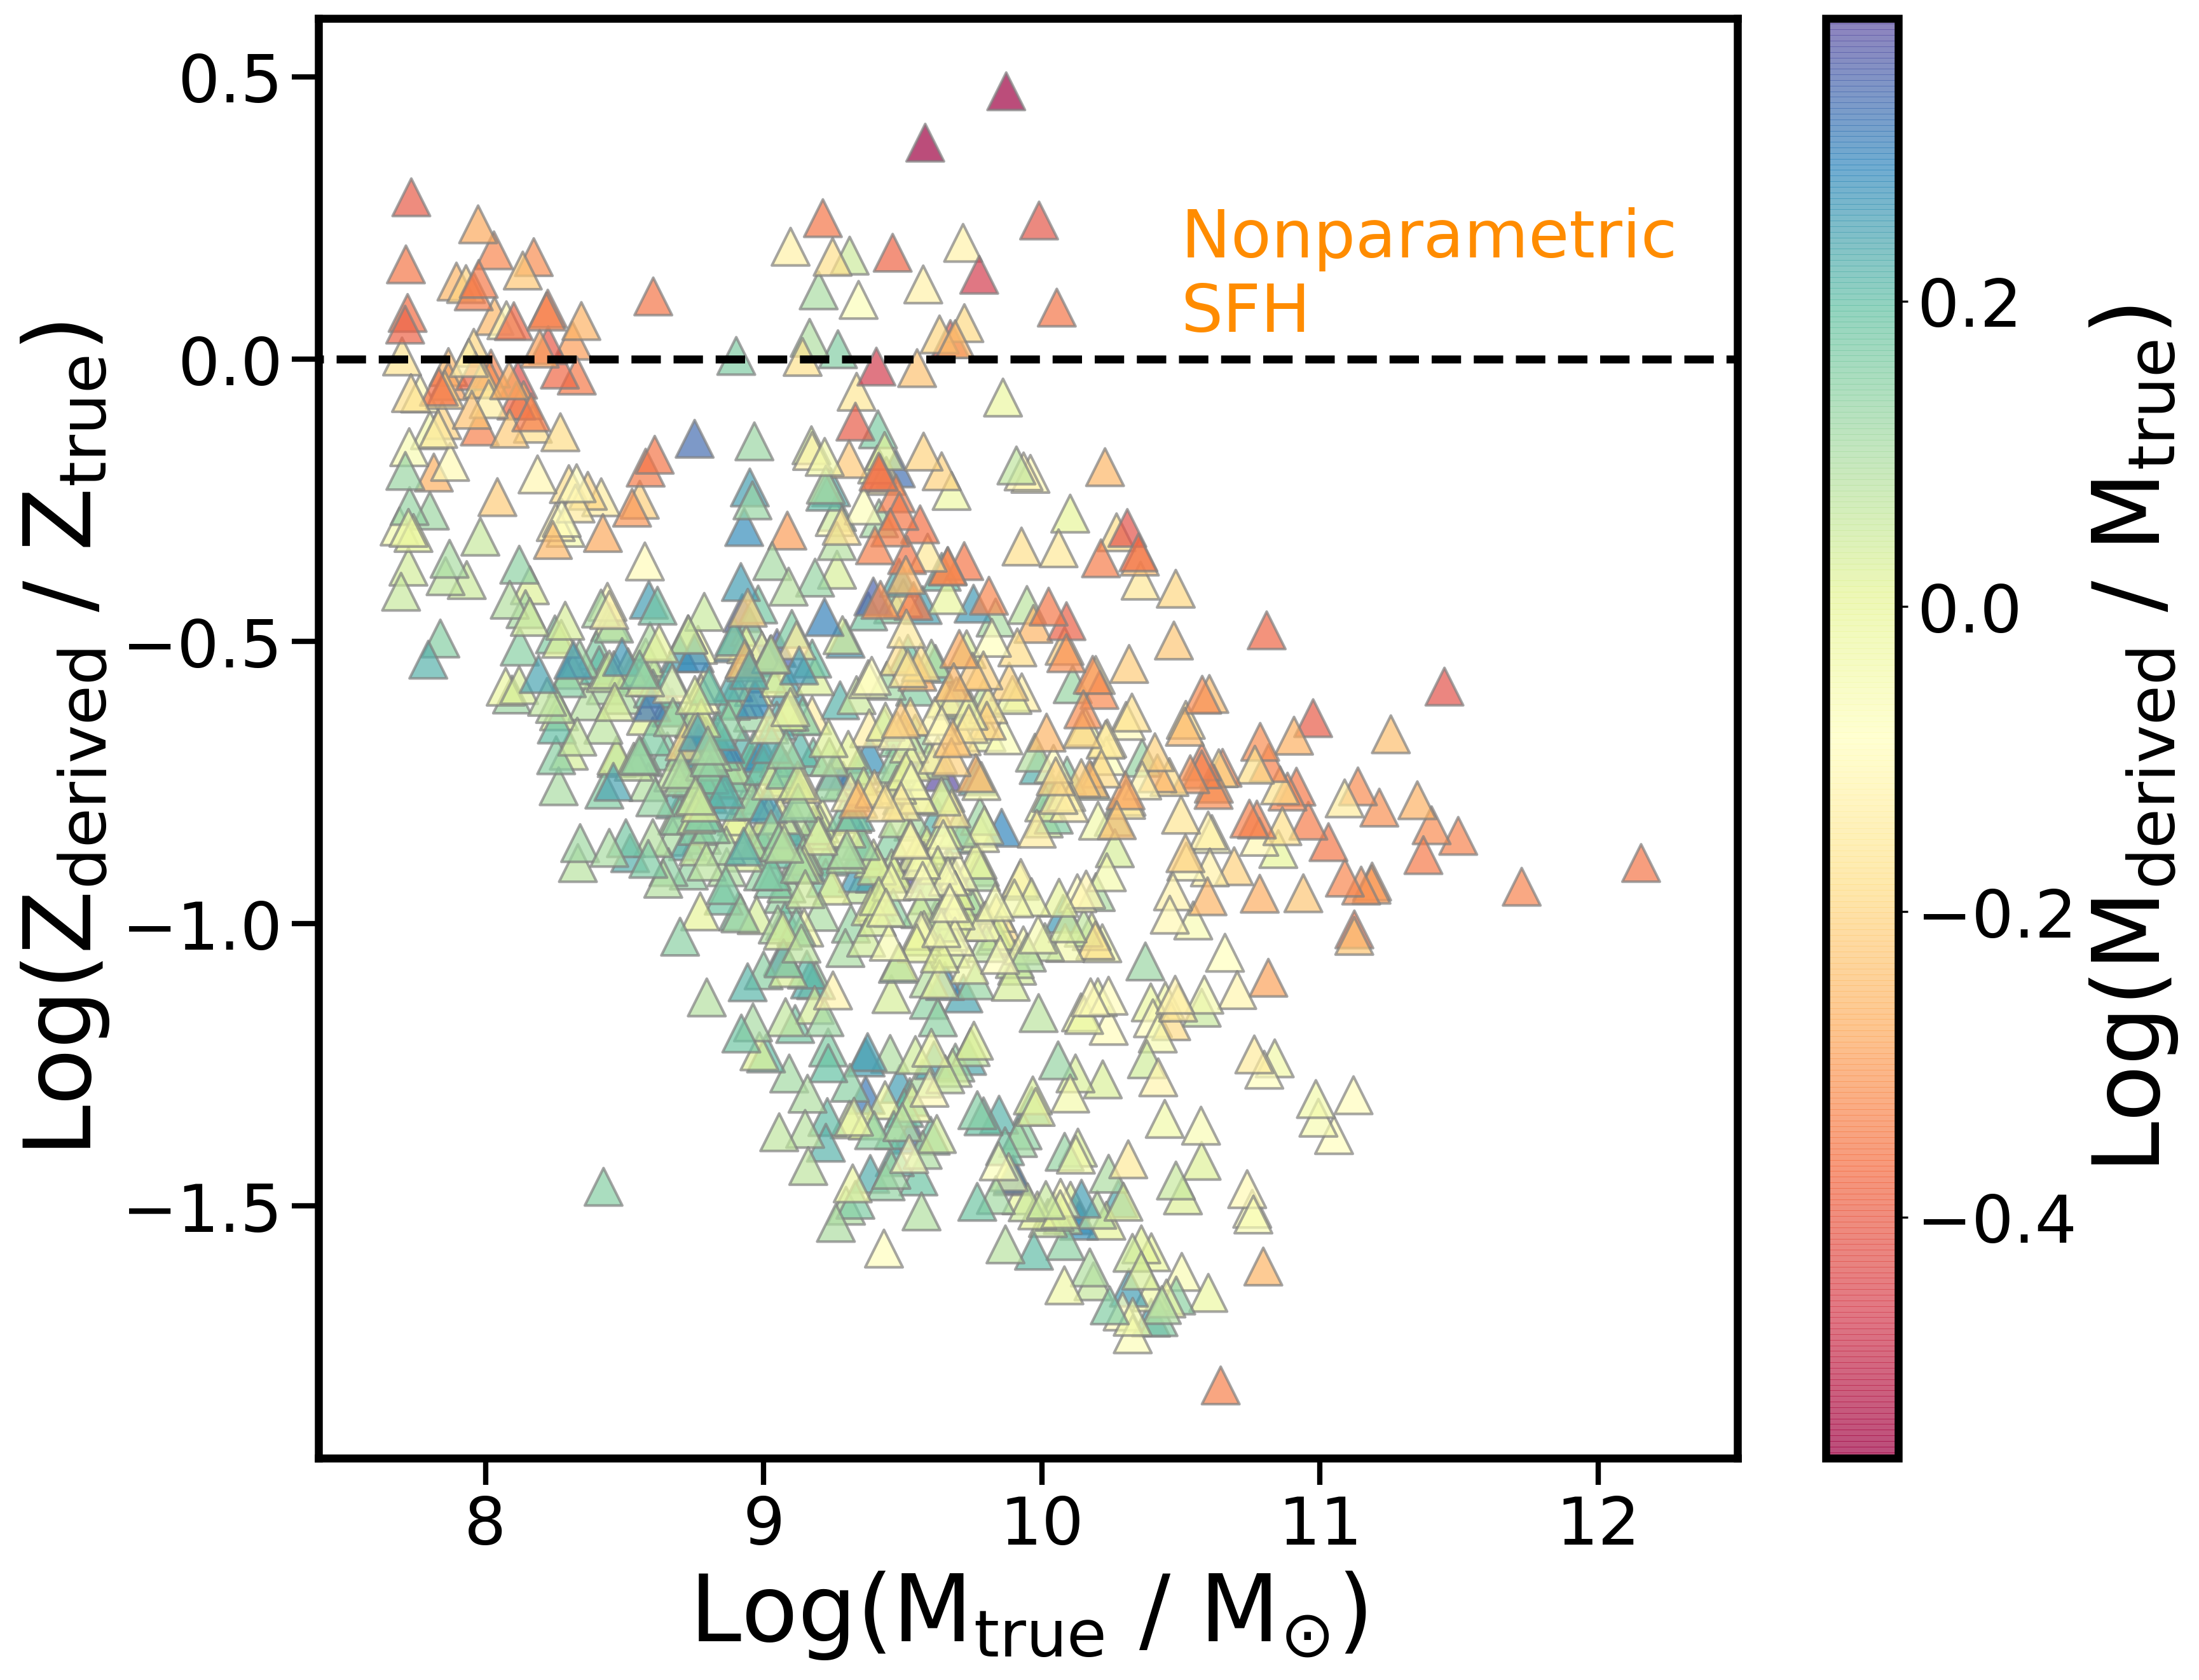
\includegraphics[width=0.49\textwidth]{Zratio_dir.png}

\caption{Correlation between the mismatches in the predicted stellar metallicity and the mismatches in the predicted stellar mass for the non-parametric model. Points are color coded according to the ratio of predicted stellar mass to true stellar mass.}
\label{fig:zratio}
\end{figure}


We find that there are systematically poor estimates for recent SFR, stellar metallicity, and dust attenuation. Each of these derived properties has an effect on the observed SED as well as on the estimated stellar masses. Additionally, the variations in one of these properties is correlated with the change in the other two, so that identical model SEDs can have vastly different associated physical properties. These model degeneracies make it difficult to accurately estimate stellar masses even with a well-sampled SED. We see that overestimates of SFR$_{10 \: \mathrm{Myr}}$ will increase the UV flux in the modeled SEDs, as a burst of recent star formation will produce massive but short-lived O and B stars that dominate the UV radiation from a galaxy over timescales of $<$ 100 Myr. Similarly, underestimating stellar metallicity will also increase the UV flux in the modeled SEDs, as lower metal content in stellar atmospheres allows for a higher escape fraction for UV photons. It should be noted, however, that \texttt{prospector} fits for the light-weighted stellar metallicity of the galaxy whereas the metallicities for the \texttt{simba} galaxies are mass-weighted. Even so, light-weighted metallicities are typically higher than mass-weighted metallicities as the light is dominated by the newer generations of stars. Dust attenuation can then be tuned in the fit to compensate for the mismatches in SFR and metallicity, demonstrating that even in the case of a reasonably well fit SED, the derived physical properties can be far from the true values and/or have large uncertainties. Indeed, the posterior distributions for model parameters in galaxies suffering from the worst stellar mass estimates were also much wider than average, indicating \texttt{dynesty}'s struggle to converge. 


We see the strong trend between the mismatch in estimated stellar metallicity and the mismatch in estimated stellar mass mentioned above and seen in Figure \ref{fig:zratio}. If \texttt{prospector} underestimates the stellar metallicity, the stellar mass is overestimated and conversely for over-estimations of stellar metallicity. Similar correlations with the mass-weighted stellar age and recent star formation rate are are not as strong, leading to the conclusion that the predicted stellar mass depends heavily on the metallicity. However, it seems more likely that the trend in metallicity can be attributed to uncertainties in the dust attenuation model. More precisely, the degeneracies between metallicities, dust attenuation, and late time star formation rate result in inaccurate model parameters. Physically, as UV light is the most affected by dust attenuation, in cases where the modeled UV SED is incorrect, the metallicity can be forced to certain values to compensate. It is also possible that the dust attenuation model used is not constrained enough by the photometric data given to produce both an accurate SED and correct physical properties. This is again due to the multitude of degeneracies that exist in SED fitting, namely that perturbing the values for stellar age, metallicity, and reddening by dust in conjunction can result in identical SEDs while the implied galaxy properties differ. Though outside the scope of discussion presented here, we can attempt to break dust attenuation model degeneracies by using cosmological simulations to constrain parameter spaces and enable the development of more flexible non-parametric dust attenuation curves. 



\section{Conclusions}

We have used simulated galaxies from the \texttt{simba} cosmological simulation to ground-truth the results of non-parametric SFHs used in SED modeling with \texttt{prospector}. These SFHs are more flexible in their ability to describe galaxy SFHs, which result in more accurate stellar mass and age estimates. We have shown that the uncertainty in stellar mass estimates decreases with the use of non-parametric SFHs, falling below a factor of 2 uncertainty, for a majority of modeled \texttt{simba} galaxies. 

The importance of more accurate stellar mass estimates cannot be understated, as many galaxy scaling relations concerning galaxy formation and evolution include stellar mass. To this end, we showed we can recover the star-forming main sequence of our galaxies to a more accurate degree than with previous parametric SFHs, matching both the intrinsic SFMS and observed galaxies from the literature. In the past, there have been tensions between observed SFR-M$_*$ relation and those calculated from simulations. As shown here and explored in \cite{katsianis_high_2020}, this tension could be the result of inaccurately estimated physical properties from SED modeling instead of intrinsic differences in the simulated physics and observations. However, these SFH models do not come without faults. We attempted to understand the cause of failed stellar mass predictions (an important note is that the 'failure' rate of the non-parametric SFHs is much less than the failure rate of the parametric models). Degeneracies between other properties and model parameters, specifically dust attenuation and stellar metallicity, and late time star formation rates can skew the stellar mass predictions away from the true values. The difficulty lies in the fact that the star formation history is only moderately constrained by broadband photometry so priors must be carefully implemented to allow a diverse range of SFHs to be modeled while simultaneously alleviating the degeneracy between other model parameters. Cosmological simulations can play an important role in future work to constrain priors not only for SFHs but also dust attenuation laws. We can also develop non-parametric models for dust attenuation in a similar way but the increase in computational resources and model degeneracies warrant caution. As such, we hope to explore further improvements to SED modeling and deriving physical properties from broadband photometry.  



\bibliographystyle{aasjournal}
\bibliography{bib2}{}




\end{document}


